%%%%%%%%%%%%%%%%%%%%%%%%%%%%%%%%%%%%%%%%%%%%%%%%%%
% Basic setup. Most papers should leave these options alone.

%\documentclass[a4paper,fleqn,usenatbib,english,doublespacing,onecolumn]{mnras}
\documentclass[a4paper,fleqn,usenatbib,english]{mnras}
\bibliographystyle{mnras}

%%%%% AUTHORS - PLACE YOUR OWN PACKAGES HERE %%%%%

%\usepackage{newtxtext,newtxmath}
\usepackage[T1]{fontenc}
\usepackage{ae,aecompl}
\usepackage[usenames,dvipsnames,svgnames,table]{xcolor}
\usepackage{hyperref}
\setcounter{tocdepth}{3}
\usepackage{amssymb}
\usepackage{amsmath}
\usepackage{relsize}
\usepackage{undertilde}
\usepackage{babel}
\usepackage{graphicx}
\usepackage{multicol}
\usepackage{bm}
\usepackage{pdflscape}
\usepackage{subfig}
\usepackage{rotating}
\usepackage{longtable}
\usepackage{bigints}
\usepackage[ruled,vlined]{algorithm2e}

\makeatletter

%%%%%%%%%%%%%%%%%%%%%%%%%%%%%%%%%%%%%%%%%%%%%%%%%%

%%%%%% AUTHORS - PLACE YOUR OWN MACROS HERE %%%%%%

\newcommand{\sn}[2]{\ensuremath{#1 \times 10^{#2}}} % Scientific notation
\newcommand{\qq}{\symbol{34}} % Straight quotes
\newcommand{\arcs}{$^{\prime\prime}$} % Arcseconds
\newcommand{\rom}[2]{\ensuremath{#1_{\mathrm{#2}}}} % Non-math subscript on term
\newcommand{\erf}{\ensuremath{\textrm{erf}}} % Error function
\newcommand{\erfc}{\ensuremath{\textrm{erfc}}} % Complementary error function
\newcommand{\ebv}{\ensuremath{E(B\,\textrm{--}\,V)}} % E(B-V)
\newcommand{\um}{$\mu$m} % microns
\newcommand{\ium}{$\mu$m$^{-1}$} % inverse microns
\newcommand{\sz}{spec-$z$} % spec-z
\newcommand{\gz}{grism-$z$} % grism-z
\newcommand{\pz}{photo-$z$} % photo-z
\newcommand{\cz}{cluster-$z$} % cluster-z

% comments
\newcommand{\alexie}[1]{\textcolor{blue}{\textbf{[Alexie: #1]}}}
\newcommand{\jean}[1]{\textcolor{orange}{{[\bf Jean: #1]}}}
\newcommand{\bl}[1]{\textcolor{green}{{[BL: #1]}}}

% edits
\newcommand{\josh}[1]{\textcolor{red}{\textbf{#1}}}

%\let\oldenumerate\enumerate \renewcommand{\enumerate}{
%	\oldenumerate
%	\setlength{\itemsep}{1pt}
%	\setlength{\parskip}{0pt}
%	\setlength{\parsep}{0pt}
%}
%
%\let\olditemize\itemize \renewcommand{\itemize}{
%	\olditemize
%	\setlength{\itemsep}{1pt}
%	\setlength{\parskip}{0pt}
%	\setlength{\parsep}{0pt}
%}

\DeclareMathAlphabet\mathbfcal{OMS}{cmsy}{b}{n} % Bold Mathcal font

%%%%%%%%%%%%%%%%%%% TITLE PAGE %%%%%%%%%%%%%%%%%%%

\title[Photo-z's with Hierarchical Bayes and Machine Learning]{Deriving Photometric Redshifts from Observed Flux Densities using Hierarchical Bayes and Machine Learning}

\author[Speagle et al.]{
	Joshua S. Speagle$^{1,2}$\thanks{E-mail: jspeagle@cfa.harvard.edu},
	Alexie Leauthaud$^{3,2}$,
	Kevin Bundy$^{3,4,2}$, 
    Peter Capak$^{5}$, \and
    Jean Coupon$^{6}$,  
	Daniel Eisenstein$^{1}$,
    Boris Leistedt$^{7}$,
	Daniel Masters$^{8}$, \and
    Daniel Mortlock$^{9,10}$,
    Hiranya Peiris$^{11,12}$
	\\
    \\
	% List of institutions
	$^{1}$Harvard University, 60 Garden St., MS 46, Cambridge, MA 02138, USA\\
	$^{2}$Kavli IPMU (WPI), UTIAS, The University of Tokyo, Kashiwanoha 5-1-5, Kashiwa, Chiba, Japan\\
	$^{3}$University of California Santa Cruz, 1156 High St., Santa Cruz, CA 95064, USA\\
	$^{4}$University of California Observatories/Lick Observatory, 1156 High St., Santa Cruz, CA 95065, USA\\
 	$^{5}$Spitzer Science Center, California Institute of Technology, Pasadena, CA 91125, USA\\
 	$^{6}$University of Geneva ch. d'Ecogia 16, CH-1290 Versoix, Switzerland\\
 	$^{7}$Center for Cosmology and Particle Physics, Department of Physics, New York University, New York, NY 10003, USA\\
     $^{8}$Infrared Processing and Analysis Center, California Institute of Technology, Pasadena, CA 91125, USA\\
     $^{9}$Astrophysics Group, Imperial College London, Blackett Laboratory, Prince Consort Road, London, SW7 2AZ, UK\\
     $^{10}$Department of Mathematics, Imperial College London, London, SW7 2AZ, UK\\
     $^{11}$Department of Physics \& Astronomy, University College London, Gower Street, London, WC1E 6BT, UK\\
     $^{12}$Oksar Klein Centre for Cosmoparticle Physics, Stockholm University, AlbaNova, SE-106 91 Stockholm, Sweden
}

% These dates will be filled out by the publisher
\date{Accepted XXX. Received YYY; in original form ZZZ}

% Enter the current year, for the copyright statements etc.
\pubyear{2016}

% Don't change these lines
\begin{document}
\label{firstpage}
\pagerange{\pageref{firstpage}--\pageref{lastpage}}
\maketitle
	
% Abstract of the paper
\begin{abstract}
We combine Bayesian inference with machine learning to derive photometric redshifts in a robust, data-driven way. By conducting targeted likelihood fitting over observed photometric probability density functions (PDFs), we show how target objects can be sparsely projected onto an arbitrary photometric basis in the presence of observational errors, missing data, and selection effects. The joint posterior between the ensemble (population) and individual (object) distributions over this basis can then be explored using hierarchical Bayesian inference. Accurate photometric redshift PDFs (along with numerous other quantities) can subsequently be computed as a by-product. Our code (\texttt{FRANKEN-Z}), its extensions, and several interactive tutorials can be found online at \url{https://github.com/joshspeagle/frankenz}.
\end{abstract}

% Select between one and six entries from the list of approved keywords.
% Don't make up new ones.
\begin{keywords}
methods: statistical -- techniques: photometric -- galaxies: distances and redshifts
\end{keywords}

%%%%%%%%%%%%%%%%%%%%%%%%%%%%%%%%%%%%%%%%%%%%%%%%%%

%%%%%%%%%%%%%%%%% BODY OF PAPER %%%%%%%%%%%%%%%%%%

\section{Introduction}
\label{sec:intro}

In the ongoing era of ``precision cosmology'', large-scale extra-galactic surveys will collect photometric data to billions of galaxies from the optical to the near-infrared (NIR) in order to measure cosmological parameters and the growth of large-scale structure to (sub-)percent level accuracy. Many of these surveys (e.g., DES\footnote{The Dark Energy Survey \citep{des05}. See \url{darkenergysurvey.org}.}, KiDS\footnote{Kilo-Degree Survey \citep{dejong+13}. See \url{kids.strw.leidenuniv.nl}.}, HSC\footnote{The Hyper Suprime-Cam \citep[HSC;][]{miyazaki+12} Subaru Strategic Program (SSP) survey (Miyazaki et al., in preparation). See \url{hsc.mtk.nao.ac.jp/ssp}.}, LSST\footnote{The Large Synoptic Survey Telescope \citep{ivezic+08}. See \url{lsst.org}.}, \textit{Euclid}\footnote{\citet{laureijs+11}. See \url{euclid-ec.org}.}, \textit{WFIRST}\footnote{The \textit{Wide-Field Infrared Surey Telescope} \citep{spergel+15}. See \url{wfirst.gsfc.nasa.gov}.}) will rely on exquisite shear measurements (e.g., from galaxy-galaxy lensing and/or cosmic shear) to meet ambitious weak lensing-oriented science goals. Due to the sensitivity of these quantities on the inferred redshift ($z$) of (1) a given galaxy and (2) the overall redshift distribution across an ensemble of galaxies, meeting the science goals for these surveys heavily depends on measuring accurate, unbiased redshifts to a significant portion of galaxies in their photometric samples.

Due to the substantial challenge of obtaining high-confidence spectroscopic redshifts (\sz's) for the majority of galaxies in the full photometric sample \citep{masters+15}, these surveys will almost entirely rely on photometric redshifts (\pz's) derived from galaxy broad-/narrow-band spectral energy distributions (SEDs).
%\footnote{While additional redshift information exists within the spatial distribution of galaxies within the sample, the use of clustering redshifts \josh{\citep[\cz's;][]{kovac+10,menard+13,aragoncalvo+15,lee+16}} are not considered here.} 
This leads to a unique set of challenges, as the sensitivity of shear measurement bias as a function of the assumed redshift requires not only accurate \pz's on average but also accurate characterization of the associated uncertainties (i.e. the full probability density function; PDF) for each individual object.

Two main techniques have been used in the literature to derive $P(z|\mathbf{\hat{F}}_g,\mathbf{\hat{C}}_g)$ for a given set of observed fluxes $\mathbf{\hat{F}}_g$ and covariances $\mathbf{\hat{C}}_g$ of a given galaxy $g$. \textbf{Template fitting} relies on deriving a set of \textit{forward mappings} and their likelihoods from a collection of ``templates'' (i.e. models) and associated (nuisance) modeling parameters to observed color space \citep[e.g.,][]{arnouts+99,benitez00,bolzonella+00,ilbert+06,cool+13,johnson+13,tanaka15}. \textbf{Machine learning}, on the other hand, uses a collection of training data to derive the best \textit{inverse mappings} from observed color space to redshift \citep[e.g.,][]{sheldon+12,carrascokindbrunner13,hoyle16,elliott+16,almosallam+16b}.

While the ``empirical'' nature and computational speed of machine learning has made it an attractive research area over the past few years \citep[see, e.g.,][for compilations of recent work]{hildebrandt+10,dahlen+13,sanchez+14}, the increasingly sophisticated use of Bayesian methods has greatly improved the information content that can be extracted from photometric data using template fitting approaches \citep{benitez00,moustakas+13}. This includes advances in properly incorporating uncertainties from both the observed photometry and input templates, prior knowledge based on previous surveys, and the development of hierarchical models that can simultaneously model the joint distribution between individual galaxies and the overall population \citep{brammer+08,tanaka15,speagleeisenstein15a,speagleeisenstein15b,leistedt+16}.

While Bayesian inference is powerful, to date applications have been limited exclusively to template-based methods. At a fundamental level, however, machine learning methods \textit{are} Bayesian in nature\footnote{This can be shown in great detail for linear regression \citep[see, e.g.,][]{hogg+10}, which represents one of the simplest applications of ``machine learning''.}, and should be interpreted as practical approximations to full Bayesian inference\citep{bishop06}. From this perspective, conducting Bayesian inference over training data rather than an underlying set of models is not only possible, but natural. Indeed, from this perspective, the difference between pre-generated sets of model photometry and training data is mostly semantics --- template-fitting methods assume a functional form for the prior/likelihood (to compute the posterior) while machine learning attempts to derive the posterior directly.

In this paper, we extend the hierarchical Bayesian formalism developed in \citet{leistedt+16} to jointly explore the probabilistic association between individual objects and the overall populations of two arbitrary datasets spanning the same domain. This allows us to extend Bayesian analysis to the types of training data more typically used in machine learning approaches. By using machine learning to generate sparse approximations to the original likelihoods, our hybrid approach simultaneously leverages the speed and data-driven nature of machine learning while retaining the statistical rigor of traditional Bayesian analysis. This represents a significant departure from previous ``hybrid'' {\pz} approaches, which have tended to focus on using Bayesian methods to combine {\pz} PDFs \textit{after} they have been computed using other methods \citep[see, e.g.,][]{carrascokindbrunner14b}.

Our sparse approximations further allows us to keep track of when, where, and how \textit{individual objects} from our training set contribute to individual and ensemble predictions. This not only allows us to decouple our original likelihoods from any posterior modifications we hope to compute later, but also enables detailed analysis of where the information content used to compute our {\pz} PDFs is coming from. We exploit these feature in Speagle et al. (in prep.) to constrain possible uncertainties in {\pz} estimation from heterogeneously populated training data using weak lensing-selected data from the HSC SSP Survey.

The outline of the paper is as follows. In \S\ref{sec:background}, we outline the fundamental connection between model-fitting and machine-learning approaches to photometric inference, discuss its application to deriving redshifts, and provide an overview of our statistical framework. In \S\ref{sec:mod}, we discuss methods for computing likelihoods in the context of different informative metrics and missing data. In \S\ref{sec:sel}, we discuss how to modify our posteriors to account for selection effects. In \S\ref{sec:pop}, we describe how to conduct basic population inference using training data and its extensions to our full hierarchical Bayesian model. In \S\ref{sec:ml_like}, we outline how machine learning can be used to approximate the true distribution from a Bayesian perspective and outline our particular application to approximating our likelihoods and posteriors. In \S\ref{sec:tests}, we demonstrate that our model performs well on mock and real data. We discuss our results in \S\ref{sec:disc}, and conclude in \S\ref{sec:conc}.

Throughout this work, boldface ($\mathbf{x}$, $\boldsymbol{\theta}$) and braces ($\lbrace x \rbrace$, $\lbrace \theta \rbrace$) are used to represent collections of elements (i.e. vectors, matrices) while italics ($x$, $\theta$) is used for singular variables and functions. All vectors used are \textit{column vectors} (i.e. $n \times 1$ matrices) unless explicitly stated otherwise. Subscripts refer to the individual subset ($\mathbf{x}_i$) or element ($\theta_i$) at that particular index ($i$). A summary of variables and some examples of notation are shown in Table \ref{tab:stats}.

All of the tests included in this paper and our code can be found online at \url{https://github.com/joshspeagle/frankenz}.\footnote{Add Zenodo link when we freeze in the version.}

%%%%%%%%%%%%%%%%%%%%%%%%%%%%%%%%%%%%%%%%%%%%%%%%%%

% \begin{table*}
% 	\centering
% 	\caption{Summary of variables and examples of notation.}
% 	\label{tab:stats}
% 	\begin{tabular}{cll} 
% 		\hline
% 		Variable & Name & Context \\
% 		\hline
% 		$\mathbf{b}$ & Bands & Collection of observed bands used to compute the photometric likelihood. \\
%         $\mathbf{\hat{C}}_g$ & Observed covariance ($g$) & The observed covariance matrix associated with galaxy $g$. \\
% 		$\lbrace \mathbf{\hat{C}}_g \rbrace$ & Observed covariance (population) & Set of observed covariance matrices in bands $\mathbf{b}$ across all galaxies indexed by $g$. \\
%         ${\hat{C}}_{g,ij}$ & Observed covariance element ($g$) & Observed covariance matrix element associated with $g$ between bands $i$ and $j$. \\
% 		$\mathbf{f}^{\mathbf{z}}$ & Population distribution & Parameterizes the population distribution over redshifts $\mathbf{z}$. \\
%         $\mathbf{\hat{F}}_h$ & Observed flux & Set of observed fluxes among bands $\mathbf{b}$ observed for $h$. \\
%         $g$ & Testing galaxy & Testing galaxy $g \in \mathbf{g}$; often used as shorthand for $(\mathbf{\hat{F}}_g,\mathbf{\hat{C}}_g)$ in PDFs.\\
% 		$\mathbf{g}$ & Testing galaxies & Collection of observed galaxies indexed by $g$. \\
%         $\gamma$ & Observed selection flag & Binary variable modeling selection effects over each $g$. \\
%         $\mathbf{h}$ & Training galaxies & Collection of training galaxies indexed by $h$. \\
%         $\boldsymbol{\eta}(g|\mathbfcal{M})$ & Nearest-neighbor selection flag & Binary vector indicating training galaxies neighboring $g$ given $\mathbfcal{M}$.\\
% 		$K_g(\mathbf{F}|\mathbf{\hat{F}}_g)$ & Kernel density & Kernel density estimate of the flux $\mathbf{F}$ in $\mathbf{b}$ associated with each $g$ given $\mathbf{\hat{F}}_g$. \\
% 		$P(z|\mathbf{\hat{F}}_g,\mathbf{\hat{C}}_g)$ & Redshift PDF & Redshift PDF for galaxy $g$ given its observed fluxes and covariances. \\
% 		$P(g|h)$ & Photometric likelihood & Photometric likelihood between $g$ and $h$ given $K_g(\mathbf{F}|\mathbf{\hat{F}}_g)$ and $K_h(\mathbf{F}|\mathbf{\hat{F}}_h)$. \\
% 		$\mathbfcal{M}$ & Machine learning ensemble & Collection of mappings $\lbrace \mathcal{M} \rbrace$ trained over Monte Carlo realizations of $\mathbf{h}$. \\
% 		$\mathbf{n}$ & Number density/counts & The number density of galaxies observed across a particular basis. \\
% 		$N_x$ & Number of elements & The size of set $\mathbf{x}$. \\
% 		$s$ & Scalefactor & Used in the scale-free version implementation of the photometric likelihood. \\
% 		$\mathbfcal{\hat{Z}}$ & Observed Bayesian evidence & The set of observed evidences $\lbrace \mathcal{\hat{Z}}_h \rbrace$ for each training object $h$ over $\mathbf{g}$. \\
% 		$z$ & Redshift & Redshift target for posterior predictions; often sampled over a discrete grid. \\
% 		\hline
% 	\end{tabular}
% 	\\
% \end{table*}

\section{Background}
\label{sec:background}

\subsection{Photometric Inference}
\label{subsec:phot_infer}

At the most basic level, {\pz}'s rely on estimating is how ``similar'' two objects $g$ and $h$ are to each other, where $g \in \mathbf{g}$ is an object from sample $\mathbf{g} = \lbrace \ldots,g,\ldots \rbrace$ with some associated observed values $\mathbf{\hat{X}}_g$ and $h \in \mathbf{h}$ is an object from sample $\mathbf{h}= \lbrace \ldots,h,\ldots \rbrace$ with observed values $\mathbf{\hat{X}}_h$. In other words, given some hypothetical galaxy $i$ with intrinsic values $\mathbf{X}_i$, we want to find out how likely we would observe both $\mathbf{\hat{X}}_g$ and $\mathbf{\hat{X}}_h$. Since we don't know what $\mathbf{X}_i$ is, however, we want to \textit{marginalize} over these quantities to find the probability that $h$ and $g$ are consistent with being the same galaxy over all possible intrinsic values of our observables.

If we assume \textit{Poisson independence} among all objects in $\mathbf{g}$ and $\mathbf{h}$, this can be written more formally as
\begin{align}
&\int P(\mathbf{\hat{X}}_g,\mathbf{\hat{X}}_h|\mathbf{X}_i) P(\mathbf{X}_i) \, d\mathbf{X}_i \equiv \int P(g,h|i^\prime) P(i^\prime) \, di^\prime \label{eq:like_general} \\ 
&= P(g,h) = P(g|h)P(h) = P(h|g)P(g) \quad . \label{eq:joint_gh}
\end{align}
where we have used our index variables $(g,h,i)$ as a stand-in for their observed features $(\mathbf{\hat{X}}_g,\mathbf{\hat{X}}_h,\mathbf{X}_i)$ and the integral over $i^\prime$ is taken over all possible \textit{realizations} of $i$ (rather than all $i \in \mathbf{i}$). We will return to this formalism in \S\ref{sec:mod}.

In practice, $\mathbf{g}$ is often a set of \textit{target} objects with \textit{unknown} properties and $\mathbf{h}$ is a set of \textit{training} objects with \textit{known} properties. We are thus interested in $P(h|g)$, which tells us the probability that our observed object $g$ is consistent with our training object $h$. Rearranging equation (\ref{eq:joint_gh}), we get \textit{Bayes theorem}
\begin{equation}
P(h|g)=\frac{P(g|h)P(h)}{P(g)}
\end{equation}
where $P(h|g)$ is the \textit{posterior} of $h$ given $g$, $P(g|h)$ is the \textit{likelihood} of $g$ given $h$, $P(h)$ is the \textit{prior} for $h$, and
\begin{equation}
P(g)=\sum_{h \in \mathbf{h}} P(g|h)P(h)
\end{equation}
is the \textit{evidence} for $g$ summed across all training objects $h \in \mathbf{h}$. Our chosen metric for computing the likelihood $P(g|h)$ is completely unspecified here, but is some function across a set of common observables between $g$ and $h$ related to equation (\ref{eq:like_general}).

From the model-fitting (i.e. template-fitting) perspective, this formalism is straightforward to interpret. Our set of ``training data'' (i.e. data where the properties of interest are known) $\mathbf{h}=\lbrace \ldots,h(\boldsymbol{\theta}_h),\ldots \rbrace$  is generated from an underlying set of models parameterized $\boldsymbol{\theta}$, our likelihood $P(g|h)=P(g|\boldsymbol{\theta}_h)$ compares the observables generated from our model with the actual observations, and our prior $P(h)=P(\boldsymbol{\theta}_h)$ is now defined over $\boldsymbol{\theta}$. We can either sample from the posterior $P(h|g)$ using ``brute-force'' tactics by fitting a set of models and their priors that were generated in advance \citep{ilbert+06,moustakas+13}, or by drawing samples directly from the posterior using, e.g., Markov Chain Monte Carlo (MCMC) methods \citep{acquaviva+11,johnson+13,speagle+16}.

Most machine learning techniques do not assign weights to the objects in their training set, implicitly assuming that they are drawn from the posterior. Training a given machine learning algorithm on given dataset thus provides ``direct access'' to the posterior via the product $P(g|h)P(h) \propto P(h|g)$. In astronomy, this assumption is almost always violated in practice due to strong selection effects, which traditionally has required some combination of reweighting, resampling, and Monte Carlo (MC) methods to try and ``massage'' the training data $\mathbf{h}$ to better approximate to the target population $\mathbf{g}$ \citep[see, e.g.,][]{lima+08}.

\subsection{Inferring Redshift from Photometry}
\label{subsec:pz_mixed}

We are interested in inferring the redshift PDF $P(z|g)$ for our observed object $g$. Given our discrete set of training objects $\mathbf{h}$, this can be factored and written as
\begin{align}
P(z|g)&=\sum_{h\in\mathbf{h}}P(z,h|g) = \sum_{h\in\mathbf{h}}P(z|h)P(h|g) \nonumber \\
&= \sum_{h\in\mathbf{h}}P(z|h)\frac{P(g|h)P(h)}{P(g)} \quad , \label{eq:pz}
\end{align}
which constitutes stacking a posterior-weighted set of underlying redshift kernels (i.e. probabilistic \textit{labels}) associated with each training object.

One often overlooked subtlety in estimate {\pz} PDFs is that $P(z|h)$---and by extension $P(z|g)$---is fundamentally a \textit{mixed distribution} as a function of \textit{object type} $t_h$. If $h$ is a star, for instance, then we know that it's true redshift $\rom{z}{true}$ is distributed as (i.e. is drawn from)
\begin{equation}
\rom{z}{true} \sim P(z|t_h=\mathrm{star}) = \delta(z=0) \quad ,
\end{equation}
which will always be located at the \textit{discrete} value $z=0$. If $h$ is a galaxy, however, then
\begin{equation}
\rom{z}{true} \sim P(z|t_h=\mathrm{gal})
\end{equation}
where $P(z|t_h=\mathrm{gal})$ is a \textit{continuous} (unknown) distribution. 

If we don't know the underlying $t_h$ for a given $h$, then our redshift kernel $P(z|h)$ must be computed by \textit{marginalizing} over $t_h$. Since $t_h$ only encompasses two discrete classes, this is simply
\begin{align}
P(z|h)&=P(t_h=\mathrm{star})\delta(z=0) \nonumber \\
&+P(t_h=\mathrm{gal})P(z|h,t_h=\mathrm{gal}) \quad .
\end{align}
By extension, our redshift PDF for $g$ can be written as
\begin{align}
P(z|g)&=\left[\sum_{h\in\mathbf{h}}P(t_h=\mathrm{star})P(h|g)\right]\delta(z=0) \nonumber \\
&+\sum_{h\in\mathbf{h}}P(t_h=\mathrm{gal})P(z|h,t_h=\mathrm{gal})P(h|g) \\
&=P(t_g=\mathrm{star})\delta(z=0) + P(z,t_g=\mathrm{gal}|h) \nonumber
\end{align}
where $P(z,t_g=\mathrm{gal}|h)=P(t_g=\mathrm{gal})P(z|h,t_g=\mathrm{gal})$ is the redshift PDF for $g$ assuming it's a galaxy.

In this paper, we will mostly focus on the more basic formalism outlined in equation (\ref{eq:pz}) and assume that $t_h = t_g = \mathrm{gal}$ for all $g \in \mathbf{g}$ and $h \in \mathbf{h}$ for convenience. We note that our overall formalism can be easily extended to incorporate this additional subtlety, and discuss cases where explicitly modeling object types becomes more important in \S\ref{sec:disc}.

\subsection{Hierarchical Inference}
\label{subsec:pop_infer}

Our overarching motivation is to compute the \textbf{probabilistic association} between our target sample $\mathbf{g}$ and our training sample $\mathbf{h}$. These can be parameterized by a set of \textit{population weights} $\mathbf{w}$ over $\mathbf{h}$, which have a corresponding PDF $P(\mathbf{w}|\mathbf{h},\mathbf{g},\mathbf{p_h})$ for a given prior $\mathbf{p_h} \equiv \lbrace \ldots,P(h),\ldots \rbrace$. The \textit{maximum-likelihood} solution to this can be shown to be\footnote{\textbf{SHOULD I INCLUDE THIS PROOF? IT'S JUST GENERALIZING THE BINNED REPRESENTATION FROM LEISTEDT+16 THEN EVALUATING EVALUATING THE PEAK OF THE RESULTING DIRICHLET.}} the Bayesian evidence for training object $h$ computed over all target objects $g$ defined as
\begin{equation}
w = \sum_{g \in \mathbf{g}} P(h|g)P(g) = p_h \sum_{g \in \mathbf{g}} P(g|h) \quad .
\end{equation}
This can be seen as the full Bayesian solution to the $k$-nearest neighbor-based reweighting scheme presented in \citet{lima+08}.

%This represents a generalization of the color-magnitude reweighting scheme presented in \citet{lima+08}. There, a variant of the $k$-nearest neighbors algorithm \citep{altman92} is used to compute an estimate sparse, approximate estimate of the evidence $\mathcal{Z}_h$ as
%\begin{equation}
%\hat{\tilde{\mathcal{Z}}}_h \equiv \sum_{H\in\mathbf{H}(g|\mathcal{M})} \tilde{P}(g|H)\tilde{P}(H)
%\end{equation}
%for each object $h$, which can be used to assign a set of \textit{population weights} $\mathbf{w}$ to our training objects via a chosen parameterization. This reweighting scheme can be seen as the \textit{maximum-likelihood} (ML) solution for the conditional probability $P(\mathbf{w}|\mathbf{h},\mathbf{g}) \approx P(\mathbf{w}|\hat{\tilde{\mathbfcal{Z}}},\mathbf{h})$.

Ideally, however, we would like to estimate our population weights along with our collection of individual posteriors $P(\mathbf{h}|\mathbf{g})$. We are thus interested in sampling a \textit{collection} of population weights $\lbrace \mathbf{w}^{(1)},\ldots,\mathbf{w}^{(n)} \rbrace$ from the \textit{joint distribution} $P(\mathbf{h},\mathbf{w}|\mathbf{g},\mathbf{p_h})$ using a \textbf{hierarchical Bayesian model}. Each set of weights then corresponds to a specific redshift population distribution and can be used to compute an updated set of posteriors, as outlined in \S\ref{sec:pop}.

%While directly sampling from the joint distribution using MCMC methods with rejection sampling-based updates \citep[e.g., standard Metropolis-Hastings updates;][]{metropolis+53,hastings70} is difficult, the conditional distributions can be easily sampled using Gibbs updates \citep{gemangeman84}. In that case, our chain draws samples by looping over $P(\mathbf{h}|\mathbf{g},\mathbf{w},\mathbf{p_h})$ and $P(\mathbf{w}|\mathbf{g},\mathbf{h},\mathbf{p_h})$.

\textbf{An important feature of our model is that this probabilistic association is conducted entirely over the \textit{observables} spanned by the discrete collection of training objects, without regards to any of the underlying (probabilistic) labels.}\footnote{Specific choices of priors might violate this assumption if they use ancillary information, but in general this is true.} As a result, once we obtain a set of samples from the joint distribution over our training set $\mathbf{h}$, we can (in theory) ``paint on'' \textit{any} underlying mapping we desire to project our samples onto the label(s) we are interested in. While in this paper we focus specifically on the $\mathbb{R}^p\rightarrow\mathbb{R}^1$ mapping from our $p$-dimensional space of observables into the 1-D space of redshift, in future work we hope to broaden this approach to multidimensional distributions encompassing ancillary physical parameters such as stellar mass.

%%%%%%%%%%%%%%%%%%%%%%%%%%%%%%%%%%%%%%%%%%%%%%%%%%

\section{Photometric Likelihoods}
\label{sec:mod}

%In \S\ref{sec:background}, we outlined the basis of our probabilistic hierarchical model. Here we describe in more detail the individual components necessary to make this work in practice. In \S\ref{subsec:like}, we derive two possible forms for the likelihood and discuss their benefits and drawbacks. In \S\ref{subsec:miss}, we discuss how to modify our likelihoods to account for missing/censored/masked data.

%To implement this in practice, however, we need to specify a likelihood function. For many datasets, the form of this function might not be known explicitly or be difficult to formulate. In those cases, machine learning can build up an ``estimate'' the likelihood function directly from the data, as outlined in \S\ref{subsubsec:dt_bayes_approx}.\footnote{While it is (generally) possible to reverse-engineer this machine learning-based estimate of the likelihood, this is seldom done in practice.} For {\pz}'s, however, we can often formulate the likelihood function explicitly. We discuss this in more detail in \S\ref{subsec:like}.

%As noted in \S\ref{subsec:ml_bayes_approx}, it is often computationally prohibitive to compute the full, brute-force likelihood. However, we also don't want to rely exclusively on machine learning because we can compute our likelihoods explicitly. Our approach to this issue is 

We wish to compute the likelihood $P(g|h)$ between galaxies $g$ and $h$ given their \textit{kernel density estimates} (KDEs) $K_g(\mathbf{F}|\mathbf{\hat{F}}_g)$ and $K_h(\mathbf{F}|\mathbf{\hat{F}}_h)$, where $\mathbf{\hat{F}}_g = \lbrace \hat{F}_{g,1},\ldots,\hat{F}_{g,n} \rbrace$ and $\mathbf{\hat{F}}_h=\lbrace \hat{F}_{h,1},\ldots,\hat{F}_{h,n} \rbrace$ are the corresponding set of $n$ observables associated with galaxies $h$ and $g$, respectively. These are most often a set of observed \textit{flux densities} within a set of bands $\mathbf{b}$, as suggested by the notation, but can also include additional observables such as a galaxy's shape or size. We will henceforth refer to them as ``flux densities'' for simplicity.

As equation (\ref{eq:like_general}), our likelihood is the convolution of these two KDEs over all possible flux densities
\begin{align}
P(g|h) &= \int P(\mathbf{F}) P(g|h,\mathbf{F}) \, d\mathbf{F} \nonumber \\
&= \int P(\mathbf{F}) K_g(\mathbf{F}|\mathbf{\hat{F}}_g) \,  K_h(\mathbf{F}|\mathbf{\hat{F}}_h) \, d\mathbf{F} \label{eq:likelihood} 
\end{align}
where $P(\mathbf{F})$ is a prior over the flux densities across $\mathbf{b}$.

\subsection{Flux Densities}
\label{subsec:like_flux}

For most galaxies, we can approximate our flux density PDFs as a multivariate Normal (i.e. Gaussian) distribution such that
\begin{equation}
K_g(\mathbf{F}|\mathbf{\hat{F}}_g) = \mathcal{N}(\mathbf{F}|\mathbf{\hat{F}}_g,\mathbf{\hat{C}}_g) \equiv \frac{\exp\left[-\frac{1}{2}||\mathbf{F}-\mathbf{\hat{F}}||_{\mathbf{\hat{C}}^{-1}}\right]}{(2\pi)^{1/2}||\mathbf{\hat{C}}_g||^{1/2}} \label{eq:mv_gauss}
\end{equation}
where
\begin{equation}
||\mathbf{F}-\mathbf{\hat{F}}||_{\mathbf{\hat{C}}^{-1}} \equiv (\mathbf{F}-\mathbf{\hat{F}}_g)^T\mathbf{\hat{C}}_g^{-1}(\mathbf{F}-\mathbf{\hat{F}}_g)
\end{equation}
is the \textit{squared Mahalanobis distance} or \textit{Mahalanobis norm} (i.e. the error-weighted distance) for vector $\mathbf{F}-\mathbf{\hat{F}}$, $\mathbf{\hat{C}}_g$ is the estimated \textit{covariance matrix}, $\mathbf{\hat{C}}_g^{-1}$ is the corresponding \textit{precision matrix}, $T$ is the transpose operator, $p$ is the total number of bands, and
\begin{equation}
||\mathbf{\hat{C}}|| \equiv ||\mathrm{vec}\left(\mathbf{\hat{C}}\right)|| = \mathrm{vec}\left(\mathbf{\hat{C}}\right)^T \mathrm{vec}\left(\mathbf{\hat{C}}\right) = \sum_{i,j} \hat{C}_{ij}^2
\end{equation}
is the Euclidean matrix norm where the $\mathrm{vec}(\cdot)$ operator ``vectorizes'' an $n \times m$ matrix by stringing it out into an $nm \times 1$ column vector.

The product of two multivariate Normal distributions $\mathcal{N}(\mathbf{F}|\mathbf{\hat{F}}_g,\mathbf{\hat{C}}_g)$ and $\mathcal{N}(\mathbf{F}|\mathbf{\hat{F}}_h,\mathbf{\hat{C}}_h)$ is a scaled multivariate Normal of the form $S_{gh}\,\mathcal{N}(\mathbf{F}|\mathbf{\hat{F}}_{gh},\mathbf{\hat{C}}_{gh})$ where
\begin{align}
S_{gh}&= \mathcal{N}(\Delta\mathbf{\hat{F}}_{gh}|\mathbf{0},\mathbf{\hat{C}}_{g+h}) \label{eq:mvg_S} \\ 
\Delta\mathbf{\hat{F}}_{gh} &\equiv \mathbf{\hat{F}}_{g}-\mathbf{\hat{F}}_{h} \\
\mathbf{\hat{C}}_{g+h}&= \mathbf{\hat{C}}_g+\mathbf{\hat{C}}_h \label{eq:mvg_C} \\
\mathbf{\hat{F}}_{gh}&= \mathbf{\hat{C}}_{gh} \left( \mathbf{\hat{C}}_g^{-1}\mathbf{\hat{F}}_g + \mathbf{\hat{C}}_h^{-1}\mathbf{\hat{F}}_h \right) \label{eq:mvg_mu} \\
\mathbf{\hat{C}}_{gh}&= \left(\mathbf{\hat{C}}_g^{-1}+\mathbf{\hat{C}}_h^{-1}\right)^{-1} \quad . \label{eq:mvg_C}
\end{align}

If we assume a uniform prior on our flux densities\footnote{This is an uninformative and improper prior linear in $\mathbf{F}$. While the ``correct'' prior would likely be logarithmic in $\mathbf{F}$, assigning such a prior would render our resulting likelihood non-analytic.} $P(\mathbf{F})=1$, then our likelihood from equation (\ref{eq:likelihood}) simplifies enormously, giving us
\begin{equation}\label{eq:likelihood_fixed}
P(g|h) = S_{gh} = \mathcal{N}(\Delta\mathbf{\hat{F}}_{gh}|\mathbf{0},\mathbf{\hat{C}}_{g+h}) \quad .
\end{equation}
The log-likelihood is then
\begin{equation}
\boxed{
-2\ln P(g|h) = ||\Delta\mathbf{\hat{F}}_{gh}||_{\mathbf{\hat{C}}_{g+h}^{-1}} + \delta 
}
\end{equation}
where
\begin{equation}
\delta \equiv N_b\ln 2\pi + \ln||\mathbf{\hat{C}}_{g+h}|| \quad ,
\end{equation}
which represents the squared Mahalanobis distance (plus a constant) between $\mathbf{\hat{F}}_g$ and $\mathbf{\hat{F}}_h$.

In the case where $\mathbf{\hat{C}}_g=\mathrm{diag}(\hat{\sigma}^2_{g,1},\ldots,\hat{\sigma}^2_{g,n})$ and $\mathbf{\hat{C}}_h=\mathrm{diag}(\hat{\sigma}^2_{h,1},\ldots,\hat{\sigma}^2_{h,n})$ are both diagonal matrices (i.e. $\mathbf{\hat{F}}_g$ and $\mathbf{\hat{F}}_h$ have fully independent errors), this reduces to
\begin{equation}
-2\ln P(g|h) = \mathlarger{\mathlarger{\sum}}_{b\in\mathbf{b}} \frac{\left(\hat{F}_{g,b}-\hat{F}_{h,b}\right)^2}{\hat{\sigma}_{g,b}^2+\hat{\sigma}_{h,b}^2} + \delta \quad .
\end{equation}

\subsection{Color Likelihoods}
\label{subsec:like_color}

While (\ref{eq:likelihood_fixed}) is analytic, straightforward to compute, and easily incorporates measurement errors from both $g$ and $h$, the explicit dependence on an object's magnitude (i.e. observed flux density) requires a training set well-populated across all relevant magnitudes and colors. 

As this requirement has historically not been available, most forward modeling-based {\pz} approaches instead introduce an additional scale-factor $\alpha$ that modifies the relevant likelihood to instead depend on similar flux \textit{ratios} (i.e. requiring objects to only have similar colors/SED shapes regardless of magnitude) to utilize a limited set of high-resolution bright templates to make predictions to faint objects. This color-based likelihood takes the form
\begin{align}
P_C(g|h) &= \int P(\mathbf{F},\alpha) \mathcal{N}(\mathbf{F}|\mathbf{\hat{F}}_g,\mathbf{\hat{C}}_g) \mathcal{N}(\mathbf{F}|\alpha\mathbf{\hat{F}}_h,\alpha^2\mathbf{\hat{C}}_h)\,d\mathbf{F}d\alpha \nonumber \\
&= \int P(\alpha) \mathcal{N}\left(\Delta\mathbf{\hat{F}}_{gh}(\alpha)|\mathbf{0},\mathbf{\hat{C}}_{g+h}(\alpha)\right)\,d\alpha \label{eq:likelihood_scalefree_general}
\end{align}
where 
\begin{align}
\Delta \mathbf{\hat{F}}_{gh}(\alpha) &\equiv \mathbf{\hat{F}}_{g} - \alpha\mathbf{\hat{F}}_{h} \\
\mathbf{\hat{C}}_{g+h}(\alpha) &\equiv \mathbf{\hat{C}}_{g}+\alpha^2\mathbf{\hat{C}}_{h}
\end{align}
and we have assumed the joint prior $P(\mathbf{F},\alpha)=P(\mathbf{F})P(\alpha)$ is separable and that $P(\mathbf{F})$ is again uniform.

As with the integral over $\mathbf{F}$, our integral over $\alpha$ will still converge under an (improper) uniform prior. In particular,
\begin{equation*}
\lim_{\alpha\rightarrow\pm\infty} \propto 1/\alpha^2 = 0, \quad \lim_{\alpha\rightarrow 0} = \mathcal{N}(\mathbf{\hat{F}}_{g}|\mathbf{0},\mathbf{\hat{C}}_{g}) = \mathrm{constant} \quad ,
\end{equation*}
which shows that our new integrand behaves like a standard Normal for small $\alpha$ but possesses inverse-quadratic rather than exponential tails. Unfortunately, however, this integral has no closed form solution and must instead be solved using numerical methods \citep[see, e.g.,][]{bertsimas+08}.

\textbf{To avoid this computational overhead, most previous approaches instead assume $\mathbf{\hat{C}}_h=0$} \citep[e.g.,][]{ilbert+06,brammer+08,sawicki12,speagleeisenstein15a,speagleeisenstein15b}. Our conditional log-likelihood $-2 \ln P_C(g|h,\alpha)$ is then quadratic in $\alpha$ (i.e. a scaled Normal), with
\begin{align}
-2 \ln P_C(g|h,\alpha) &= ||\Delta\mathbf{\hat{F}}_{gh}(\alpha)||_{\mathbf{\hat{C}}_g^{-1}} + \delta_c \\
&=\frac{\rom{\alpha}{ML}^2}{\gamma^2} (\alpha^\prime-1)^2 - 2\ln P_C(g|h,\rom{\alpha}{ML}),
\end{align}
where $\alpha^\prime\equiv\alpha/\rom{\alpha}{ML}$ is the ML-normalized scalefactor and $\gamma/\rom{\alpha}{ML}$ is the associated \textit{shapefactor} (i.e. the ``standard deviation''). Solving for $\rom{\alpha}{ML}$ and $\gamma$, we get
\begin{align}
\rom{\alpha}{ML}&=\frac{\gamma^2}{2}\left(\mathbf{\hat{F}}_g^T\mathbf{\hat{C}}_g^{-1}\mathbf{\hat{F}}_h + \mathbf{\hat{F}}_h^T \mathbf{\hat{C}}_g^{-1} \mathbf{\hat{F}}_g\right) \label{eq:chi2_s_ml} \\
\gamma &= \left(\mathbf{\hat{F}}_h^T\mathbf{\hat{C}}_g^{-1}\mathbf{\hat{F}}_h^T\right)^{-1/2}.
\end{align}

Marginalizing over $\alpha^\prime$, our color-based likelihood\footnote{Our choice to marginalize over $\alpha^\prime$ instead of $\alpha$, leading to an additional $\rom{\alpha}{ML}^2$ term in our likelihood, is to normalize our results to the ML-scale such that objects with similar colors but different magnitudes (and thus different scalefactors $\alpha$) are considered more or less equally likely.} is then
\begin{equation}\label{eq:likelihood_scaled_pdf_model_mod}
P_C(g|h)=\mathcal{N}(\Delta\mathbf{\hat{F}}_{gh}(\rom{\alpha}{ML})|\mathbf{0},\mathbf{\hat{C}}_g)\left(\frac{2\pi\gamma^2}{\rom{\alpha}{ML}^2}\right)^{\frac{1}{2}}
\end{equation}
with log-likelihood
\begin{equation}
\boxed{
-2 \ln P_C(g|h) = ||\Delta\mathbf{\hat{F}}_{gh}(\rom{\alpha}{ML})||_{\mathbf{\hat{C}}_g^{-1}} + \delta_C
}
\end{equation}
where
\begin{equation}
\delta_C \equiv (N_b-1)\ln 2\pi + \ln||\mathbf{\hat{C}}_g|| + 2\ln \frac{\rom{\alpha}{ML}}{\gamma} \quad .
\end{equation}

For independent errors, this reduces to
\begin{equation}
-2\ln P_C(g|h) = \mathlarger{\mathlarger{\sum}}_{b\in\mathbf{b}} \frac{\left(\hat{F}_{g,b}-\rom{\alpha}{ML}\hat{F}_{h,b}\right)^2}{\hat{\sigma}_{g,b}^2} + \delta_C \quad ,
\end{equation}
which resembles the more familiar ``$\chi^2$ statistic'' (plus a constant) often cited in {\pz} model-fitting papers.

\subsection{Dealing with Missing Data}
\label{subsec:miss}

In practice, our unknown galaxy $g$ and training galaxy $h$ might not be observed in the exact same bands. More formally, this implies that the overlapping bands $\mathbf{b}_{gh}$ between $\mathbf{b}_g$, the bands $g$ is observed in, and $\mathbf{b}_h$, the bands $h$ is observed in, are a subset of $\mathbf{b}$ such that $\mathbf{b}_{gh} \equiv \mathbf{b}_g \cap \mathbf{b}_h \subseteq \mathbf{b}$. 

Because our likelihoods can only be computed in overlapping bands, this is equivalent to introducing a $p \times 1$ \textit{band mask} vector $\boldsymbol{\beta}(g|h)$ over our $p$ bands that evaluates to one for $b \in \mathbf{b}_{gh}$ and zero otherwise. Assuming our observed flux densities and associated covariances are always defined over all bands and defining 
\begin{equation}
\underline{\mathbf{\hat{C}}}_{g}^{-1} \equiv \mathbf{B}(g|h) \bullet \mathbf{\hat{C}}_{g}^{-1}
\end{equation}
to be the masked precision matrix given
\begin{equation}
\mathbf{B}(g|h) \equiv \left[\boldsymbol{\beta}(g|h)\right]\left[\boldsymbol{\beta}(g|h)\right]^T \quad ,
\end{equation}
our original likelihoods can be rewritten as
\begin{align}
&-2 \ln P(g|h) = ||\Delta\mathbf{\hat{F}}_{gh}||_{\underline{\mathbf{\hat{C}}}_{g+h}^{-1}} + \underline{\delta} \\
&-2 \ln P_C(g|h) = ||\Delta\mathbf{\hat{F}}_{gh}(\rom{\alpha}{ML})||_{\underline{\mathbf{\hat{C}}}_{g}^{-1}} + \underline{\delta}_C
\end{align}
where $\underline{\delta}$ and $\underline{\delta}_C$ have also absorbed changes from the inclusion of the band mask.

The changing number of bands introduces several complications into our likelihood calculation. First, it harshly penalizes adding additional dimensions, as both the Mahalanobis distance (the main portion of our likelihood computation) and the normalization (from our multivariate Gaussian) increase with the number of dimensions. This means that, \textit{for the exact same training/target galaxy pair}, our original likelihoods would tend to favor a solution with fewer bands (more masking) than one with more bands (less masking). Intuitively, we expect these should give similarly good fits, so this is clearly undesirable behavior. By extension, this makes it difficult to properly compare likelihoods between training/target galaxy pairs with varying numbers of bands, which are important for properly computing posteriors and population weights.

To correct for this, we need to examine how our likelihood changes as the number of available bands (i.e. the dimensionality of the fit) changes. In particular, for $\mathbf{\hat{X}}$ distributed as (i.e. drawn from) a $d$-dimensional multivariate Normal with mean vector $\boldsymbol{\mu}$ and covariance matrix $\mathbf{C}$, the square Mahalanobis distance between $\mathbf{\hat{X}}$ and $\mathbf{0}$ is distributed as a \textit{non-central chi-square} $\chi^2_p(\lambda=||\boldsymbol{\mu}||_{\mathbf{C}^{-1}})$ with $p$ degrees of freedom and non-centrality parameter $\lambda$. More formally,
\begin{equation}
\mathbf{\hat{X}} \sim \mathcal{N}_{p}(\mathbf{X}|\boldsymbol{\mu},\mathbf{C}) \Rightarrow
\mathbf{\hat{X}}^T\mathbf{C}^{-1}\mathbf{\hat{X}} \sim \chi^2_p(\lambda=||\boldsymbol{\mu}||_{\mathbf{C}^{-1}}) \quad .
\end{equation}

Going back to equation (\ref{eq:mvg_S}), we see that our expression for $S_{gh}$ is simply the likelihood of $\Delta\mathbf{\hat{F}}_{gh}$ assuming $\Delta\mathbf{\hat{F}}_{gh} \sim \mathcal{N}(\Delta\mathbf{F}_{gh}|\mathbf{0},\mathbf{\hat{C}}_{h+g})$. This implies that
\begin{align}
||\Delta\mathbf{\hat{F}}_{gh}||_{\underline{\mathbf{\hat{C}}}_{g+h}^{-1}} &\sim \chi^2_p(\lambda) \\
||\Delta\mathbf{\hat{F}}_{gh}(\rom{\alpha}{ML})||_{\underline{\mathbf{\hat{C}}}_g^{-1}} &\sim \chi^2_{p-1}(\lambda_C)
\end{align}
where $p=\sum_{b\in\mathbf{b}}\beta_b(g|h)$ is the number of bands used in the fit (i.e. the dimensionality) and the non-centrality parameters $\lambda$ and $\lambda_C$ are unknown.\footnote{The change from $d$ to $d-1$ comes from removing a degree of freedom when solving for $\rom{\alpha}{ML}$.} Our original likelihoods are thus distributed as
\begin{align}
-2\ln P(g|h) &\sim \chi^2_p(\lambda_p + \delta_p) \\
-2 \ln P_C(g|h) &\sim \chi^2_{p-1}(\lambda_{C,p-1} + \delta_{C,p-1})
\end{align}
where we have added in $p$ subscripts to indicate all of our non-centrality parameters are also (monotonically increasing) functions of the dimensionality $p$.

To more clearly illustrate the behavior of our likelihoods as a function of dimensionality, we note that the expectation value of our likelihood is
\begin{equation}
E\left[ -2 \ln P(g|h) \right] = p + (\lambda_p + \delta_p) \quad ,
\end{equation}
which scales as the number of bands in our fit $p$ both directly (via $p$) and indirectly (via $\lambda_p$ and $\delta_p$). Again, this is clearly undesirable since we would like for our likelihoods to be (approximately) band-invariant rather than growing super-linearly in $p$.

To define ``band-invariant'' likelihoods, we want to shift our perspective from an absolute to a relative goodness-of-fit metric. In other words, rather than comparing the likelihood of $g$ given $h$ absent any context, we want to ask how much \textit{better} $h$ is relative to the assumption that $h$ is actually a Monte Carlo realization $g^\prime$ of $g$. This modified log-likelihood (ratio) is then distributed as the convolution of two independent non-central chi-square distributions
\begin{equation}
-2 \ln P(g|h) \sim \chi^2_p(\lambda_p + \delta_p) - \chi^2_p(\delta_p)
\end{equation}
with expectation value $E\left[-2 \ln P(g|h)\right] = \lambda_p$. This new likelihood is thus an unbiased probe of the true non-centrality (i.e. ``mis-centering'') of our fit, and for a given $\lambda_p$ and $\delta_p$ we can directly compare our results across bands.

Unfortunately, $\lambda_p$ is unknown (by construction). While we could theoretically compute
\begin{equation}
P(g|h) = \int P(\lambda_p) P(g|h,\delta_p,\lambda_p) \, d\lambda_p
\end{equation}
by numerically marginalizing over $\lambda_p$, this would break our original analytic formalism. Implementing a first-order correction, however, is extremely straightforward since $E\left[\chi^2_p(\delta_p)\right]=p+\delta_p$. Our new approximate \textbf{band-invariant likelihoods} then are
\begin{equation}\label{eq:like_flux_bandinv}
\boxed{
-2\ln P(g|h) \equiv ||\Delta\mathbf{\hat{F}}_{gh}||_{\underline{\mathbf{\hat{C}}}_{g+h}^{-1}} - p
}
\end{equation}
in flux density and
\begin{equation}\label{eq:like_color_bandinv}
\boxed{
-2 \ln P_C(g|h) \equiv ||\Delta\mathbf{\hat{F}}_{gh}(\rom{\alpha}{ML})||_{\underline{\mathbf{\hat{C}}}_g^{-1}} - (p-1)
}
\end{equation}
in color.

Our choice to only implement a first-order correction means that although the likelihoods above are band-invariant \textit{on average}, their higher-order moments are not. We find the possible biases this assumption introduces to be negligible during our tests (see \S\ref{sec:tests}), but note that this might not hold true in general.

%We note that for a fixed number of bands, our band-invariant likelihoods reproduce the likelihoods presented in previous papers up to a scaling factor that is constant across all objects. We thus find that previous approaches \textit{have already been implicitly making the assumptions we explicitly derive here}.

\section{Selection effects}
\label{sec:sel}

In general, we have often \textit{selected} our sample $\mathbf{g}$ through a series of implicit and explicit \textit{selection functions}, which may be different from those used to select our training sample $h$ \citep[cf.][]{daylan+16}. One concrete instance of this is for applications to weak lensing science for current/upcoming surveys such as HSC and \textit{Euclid}, where (1) the training sample $\mathbf{h}$ is observed at deeper depths than the overall survey and (2) the galaxies $\mathbf{g}$ used for weak lensing-oriented science are often selected to have significantly higher signal-to-noise than the general survey.

Following \citet{leistedt+16} we can define an $N_g \times 1$ \textit{sample selection mask} vector $\mathbf{s}(\mathbfcal{S})$ over $\mathbf{g}$ as a function of the selection criteria $\mathbfcal{S}=\lbrace \mathcal{S}_1, \ldots, \mathcal{S}_n \rbrace$ used to construct $\mathbf{g}$. This is analagous to our band mask defined in \S\ref{subsec:miss}, where $s_g=1$ for $g \in \mathbf{g}$ selected and $0$ otherwise. Note that, by design, $\mathbf{s}(\mathbfcal{S})=\mathbf{1}$.

Conditioning on $\mathbfcal{S}$, we are now interested in estimating the posterior conditioned on $s_g=1$, $P(h|g,s_g=1,\mathbfcal{S})$, which is the probability that $g$ is consistent with $h$ given that $g$ has been selected in our sample. Our target posterior is then
\begin{equation}
\boxed{
P(h|g,s_g=1,\mathbfcal{S}) = \frac{P(s_g=1|h,\mathbfcal{S}) P(h|g)}{P(s_g=1|\mathbfcal{S})}
} \quad ,
\end{equation}
where 
\begin{equation}
P(s_g=1|\mathbfcal{S}) = \sum_{h \in \mathbf{h}} P(s_g=1|h,\mathbfcal{S}) P(h|g)
\end{equation}
and our \textit{selection probability} $0 \leq P(s_g=1|h,\mathbfcal{S}) \leq 1$ is defined as
\begin{equation}\label{eq:sel_g_h}
P(s_g=1|h,\mathbfcal{S}) = \frac{\int P(s_g=1|g^\prime,\mathbfcal{S}) P(g^\prime|h) \, dg^\prime}{\int P(g^\prime|h) \, dg^\prime} \quad ,
\end{equation}
where the integral over $g^\prime$ is taken over all possible realizations of $g$. Note that this integral often cannot be solved analytically and must be computed using numerical methods.

%\footnote{While not explicitly discussed here, we wish to note that this methodology can in theory also be applied to the training sample, whereby a combination of priors combined with knowledge of the selection function can be used to derive Bayesian posterior estimates for our KDEs $K_h(\mathbf{F}|\mathbf{\hat{F}}_h,\mathbf{\hat{C}}_h$. This, however, will break our multivariate normal assumption and render our original likelihoods non-analytic.}

We emphasize that this derivation is completely agnostic to our selection criteria $\mathbfcal{S}$ and the corresponding selection probability $P(s_g=1|g^\prime,\mathbfcal{S})$. In particular, there are no requirements that
\begin{itemize}
	\item $P(s_g=1|g^\prime,\mathbfcal{S})$ and/or $P(s_g=1|h,\mathbfcal{S})$ are analytic,
    \item $P(s_g=1|g^\prime,\mathbfcal{S})$ is separable, and/or
    \item $P(s_g=1|g^\prime,\mathbfcal{S})$ is a strict binary cut.\footnote{A good example of a non-binary selection effect might be where our observables serve only as a (probabilistic) proxy for a cut is being applied via a set of variables we do not (currently) have access to.}
\end{itemize}

These specific cases, however, often do arise in practice, and properly exploiting them can dramatically simplify the process of computing our selection probability. We outline several examples using flux density cuts in \S\ref{subsec:sel_flux} below. For completeness, we also outline a more general case involving color cuts in \S\ref{subsec:sel_color}.

\subsection{Flux Density Cuts}
\label{subsec:sel_flux}

\subsubsection{Magnitude Cuts}
\label{subsubsec:sel_mag}

The simplest types of selection effects are those that operate directly on our flux densities (i.e. our observables). These are most often imposed as a \textit{magnitude cut} corresponding to a specific flux density cutoff $\rom{\mathbf{F}}{cut}$, and can be parameterized by
\begin{equation}
P(s_g=1|g^\prime,\rom{\mathcal{S}}{mag})=\mathcal{H}(\mathbf{\hat{F}}^\prime_g-\rom{\mathbf{F}}{cut})
\end{equation}
where
\begin{equation}
\mathcal{H}(\mathbf{x}) \equiv \prod_{b\in\mathbf{b}} \mathcal{H}(x_b)
\end{equation}
is the ``vectorized'' \textit{Heavyside function}, which evaluates to $1$ for $\mathbf{x} \geq 0$ element-wise and $0$ otherwise. Our selection probability then becomes
\begin{equation}
P(s_g=1|h,\rom{\mathcal{S}}{mag}) = \frac{\int_{\mathbf{F}>\rom{\mathbf{F}}{cut}} P(g^\prime|h) \, dg^\prime}{\int P(g^\prime|h) \, dg^\prime} \quad .
\end{equation}
%In the limit of $\rom{\mathbf{F}}{cut}=\lbrace -\infty, \ldots, -\infty \rbrace$, this evaluates to $P(s_g|h,\rom{\mathcal{S}}{mag})=1$ for all galaxies, as expected.

If we assume we are working with the likelihoods defined via equations (\ref{eq:like_flux_bandinv}) or (\ref{eq:like_color_bandinv}), then $P(g^\prime|h)$ simply represents a scaled multivariate Gaussian. Our selection probability then can be seen as the complement of the cumulative distribution function (CDF) of this multivariate Gaussian (i.e. the chance of \textit{not} having our galaxy below our magnitude cut). If we assume that our covariance matrix is diagonal, the complement of the multivariate CDF factors into the product of the complements of the CDFs of univariate Gaussians. These can be parameterized by
\begin{align}
\Phi_c(x|\mu,\sigma^2) &\equiv 1-\Phi(x|\mu,\sigma^2) \equiv \int_{x}^{+\infty} \mathcal{N}(x|\mu,\sigma^2) \nonumber \\
&= 1 - \frac{1}{2}\,\erfc\left(\frac{\mu-x}{\sqrt[]{2}\sigma}\right) \quad,
\end{align}
where $\erfc$ is the \textit{complementary error function}. 

Assuming our likelihoods are defined directly from our flux densities as equation (\ref{eq:like_flux_bandinv}), our final expression for the selection probability introduced by $\rom{\mathcal{S}}{mag}$ is
\begin{align}
P(s_g=1|h,\rom{\mathcal{S}}{mag}) &= \mathlarger{\prod}_{b\in\mathbf{b}} \Phi_c \left( F_{\mathrm{cut},b} | \hat{F}_{h,b}, \hat{\sigma}^2_{g,b}+\hat{\sigma}^2_{h,b} \right) \quad .
%P_C(s_g|h,\rom{\mathcal{S}}{mag}) &= \mathlarger{\prod}_{b\in\mathbf{b}} \Phi_c \left( F_{\mathrm{cut},b} | \rom{\alpha}{ML}\hat{F}_{h,b}, \hat{\sigma}^2_{g,b} \right)
\end{align}
%for our flux density and color-based likelihoods, respectively.

\subsubsection{Signal-to-Noise Cuts}
\label{subsubsec:sel_sn}

With this function as a baseline, we can easily construct the selection probabilities for a signal-to-noise (S/N) cut. Note that a S/N cut is functionally equivalent to a flux density cut for each individual object, but where the cut is a function of the measurement error. For a S/N threshold $X$, this gives
\begin{equation}
P(s_g=1|h,\rom{\mathcal{S}}{S/N}) = \mathlarger{\prod}_{b\in\mathbf{b}} \Phi_c \left( X\hat{\sigma}_{g,b} | \hat{F}_{h,b}, \hat{\sigma}^2_{g,b}+\hat{\sigma}^2_{h,b} \right) \quad .
\end{equation}

By building on these baseline cases with judicious application of logical statements and the \textit{inclusion-exclusion principle}, more complex cuts can be constructed. For instance, photometric extraction thresholds are typically a logical combination of individual S/N cuts, where photometry for a galaxy is extracted if it is detected above a S/N threshold $X$ in $\geq Y$ bands. In the case $Y=1$, we note that the probability of detecting a given galaxy with S/N $\geq X$ in \textit{more than} one band is the complement of the probability of observing with S/N $\geq X$ in \textit{no} bands. This gives
\begin{equation}
P(s_g=1|h,\rom{\mathcal{S}}{det}) = 1 - \mathlarger{\prod}_{b\in\mathbf{b}} \Phi \left( X\hat{\sigma}_{g,b} | \hat{F}_{h,b}, \hat{\sigma}^2_{g,b}+\hat{\sigma}^2_{h,b} \right) \quad .
\end{equation}

Note that our various selection cuts contained within $\mathbfcal{S}$ might or might not be fully independent of each other. For instance, if we impose magnitude cuts in two \textit{separate} bands $b_1$ and $b_2$, our corresponding selection probabilities are independent and $P(s_g=1|h,\mathbfcal{S}) = P(s_g=1|h,\mathcal{S}_{b_1}) \times P(s_g=1|h,\mathcal{S}_{b_2})$. However, if we are instead imposing a magnitude and S/N cut in the \textit{same} band $b$, then our flux density threshold used to compute $P(s_g=1|h,\mathbfcal{S})$ instead becomes $\rom{F}{eff,b}=\max\left\lbrace \rom{F}{cut,b}, X\hat{\sigma}_{g,b} \right\rbrace$.

If we are concerned with keeping our selection probability in a (pseudo-)analytic form, thinking carefully about these issues is critical to ensuring our final result is consistent with our original set of selection criteria. As discussed in the next section, however, there always isn't a simple functional form for $P(s_g|h,\mathcal{S})$, at which point these issues become less critical to resolve because we are forced to evaluate our integrals numerically regardless.

\subsection{Color Cuts}
\label{subsec:sel_color}

Outside of magnitude cuts, a common way to select interesting (sub)samples of objects from parent survey populations involves imposing a series of color cuts, which can be interpreted as cuts across a given (unique) collection of \textit{flux density ratios}
\begin{equation}
\mathbf{\hat{R}}_g \equiv \left\lbrace \hat{F}_{g,i}/\hat{F}_{g,j} \,\, \forall \,\, j>i \right\rbrace \quad .
\end{equation}

Our selection function can again be modeled as a Heavyside function evaluated element-wise across $\mathbf{\hat{R}}_g$ such that
\begin{equation}
P(s_g=1|g^\prime,\rom{\mathcal{S}}{color}) = \mathcal{H}(\mathbf{\hat{R}}_g^\prime-\rom{\mathbf{R}}{cut}),
\end{equation}
where $\mathbf{\hat{R}}_g^\prime$ is generated from $\mathbf{\hat{F}}_g^\prime$. Unfortunately, there is no analytic form for the corresponding integral over $\mathbf{R}$, requiring us to resort to numerical integration techniques to evaluate $P(s_g=1|h,\rom{\mathcal{S}}{color})$.

The most straightforward numerical integration method here is \textit{importance sampling}. For a series of $n$ Monte Carlo realizations $\left\lbrace \mathbf{\hat{F}}_g^{(1)},\ldots,\mathbf{\hat{F}}_g^{(n)} \right\rbrace$ of the flux density of galaxy $g$ labeled as
\begin{equation}
\left\lbrace g^{(1)},\ldots,g^{(n)} \right\rbrace \sim Q(g|h)
\end{equation}
drawn from a prior distribution $Q(g|h)$ designed to approximate $P(g|h)$, we can approximate our original integral as
\begin{align}
&\int P(s_g=1|g^\prime,\mathbfcal{S}) P(g^\prime|h) \, dg^\prime \nonumber \\ 
&\approx \frac{1}{n} \sum_{i=1}^n w(g^{(i)}|h) P(s_g=1|g^{(i)},\mathbfcal{S})
\end{align}
where 
\begin{equation}
w(g^{(i)}|h) \equiv \frac{P(g^{(i)}|h)}{Q(g^{(i)}|h)}
\end{equation}
is the associated \textit{importance weight} for the $i$th sample. 

For our flux density and color-based likelihoods defined in equations (\ref{eq:like_flux_bandinv}) and (\ref{eq:like_color_bandinv}), we can sample directly from $P(g^\prime|h)$. Our importance weights then become unity such that $w(g^{(1)}|h)=\ldots=w(g^{(N)}|h)=1$, and our numerical integration becomes a simple counting exercise of how frequently our samples $g^{(i)}$ meet our selection criteria. It is not always possible to sample directly from more complex likelihoods such as, e.g., equation (\ref{eq:likelihood_scalefree_general}), however, and so we keep the full derivation above for generality.

%%%%%%%%%%%%%%%%%%%%%%%%%%%%%%%%%%%%%%%%%%%%%%%%%%

\section{Hierarchical Inference}
\label{sec:pop}

We now want to broaden our individual posteriors from \S\ref{sec:sel} to incorporate population information using a \textbf{hierarchical Bayesian model}. In \S\ref{subsec:ideal}, we outline a simple case of how to conduct population inference in 1-D given a sample of known redshifts. In \S\ref{subsec:obs}, we broaden our framework to $p$-dimensional inference over photometric observables including selection effects. In \S\ref{subsec:hier}, we describe our full hierarchical model.

\josh{ADD OVERVIEW FIGURE FOR FRAMEWORK+IMPLEMENTATION.}

\subsection{Population Inference with Redshifts (1-D)}
\label{subsec:ideal}

Let's first assume that instead of photometry, for each unknown galaxy $g \in \mathbf{g}$ and training galaxy $h \in \mathbf{h}$ we have a 1-D redshift PDF characterized by $K_g(z|\hat{z}_g)$ and $K_h(z|\hat{z}_h)$, respectively, where $\hat{z}_i$ is the ``observed'' redshift. For a set of \textit{population weights} $\mathbf{w}$ our redshift \textit{population distribution} can be expressed as 
\begin{equation}\label{eq:pz_pop}
P( z | \lbrace \mathbf{h},\mathbf{w} \rbrace ) = \left. \sum_{h \in \mathbf{h}} w_h K_h(z|\hat{z}_h) \middle/ \sum_{h \in \mathbf{h}} w_h \right.
\end{equation}
where $\mathbf{w}$ is an implicit function of (at the minimum) $\mathbf{g}$ and $\mathbf{h}$.

One possible choice for $w_h$ is the Bayesian evidence $\mathcal{Z}_h$ for $h$ computed over all $g \in \mathbf{g}$, defined as
\begin{equation}
\mathcal{Z}_h \equiv \sum_{g \in \mathbf{g}} P(h|g) P^\prime(g) \quad .
\end{equation}
In this symmetric representation of our original posteriors defined over $\mathbf{h}$, $P^\prime(g)$ no longer represents the evidence from our original fit $P(g)$ but rather a \textit{prior weight} for object $g$. Defining these prior weights over $\mathbf{g}$ as $\mathbf{p}=\lbrace \ldots, P^\prime(g), \ldots \rbrace$ and our original set of priors over $\mathbf{h}$ as $\mathbf{q}=\lbrace \ldots, P(h), \ldots \rbrace$, our evidence becomes
\begin{equation} \label{eq:evidence}
\mathcal{Z}_h \equiv \sum_{g \in \mathbf{g}} p_g \times \frac{q_h P(g|h)}{\sum_{h \in \mathbf{h}} q_h P(g|h)}
\end{equation}
where our likelihood is now
\begin{equation}
P(g|h) = \int P(z) K_g(z|\hat{z}_g) K_h(z|\hat{z}_h) \, dz \quad .
\end{equation}
This is a specific case of our generalized likelihood outlined in equation (\ref{eq:likelihood}) evaluated over a given redshift prior $P(z)$.

This formulation of the Bayesian evidence constitutes a fully probabilistic generalization of the projected number densities typically used in the literature. We can recover the histogrammed redshift number densities used more commonly in the literature by making the following assumptions:
\begin{enumerate}
    \item the redshift PDFs $K_g(z|\hat{z}_g) = \delta(z-\hat{z}_g)$ for $g \in \mathbf{g}$ are perfectly measured they are effectively delta functions,
    \item our prior weights $\mathbf{p}$ over $\mathbf{g}$ are uniform,
    \item the redshift PDFs $K_h(z|\hat{z}_h) = \Theta\left(z - \hat{z}_h^{-}\right) \Theta\left(\hat{z}_h^{+} - z\right)$ for $h \in \mathbf{h}$ are a series of histogram bins with bin centers $\hat{z}_h$ and widths $\Delta \hat{z}_h$, where $\hat{z}_h^{\pm} \equiv \left(\hat{z}_h \pm \Delta\hat{z}_h\right)/2$,
    \item our prior $\mathbf{q}$ over $\mathbf{h}$ is uniform, and
    \item our redshift prior $P(z)$ is uniform.
\end{enumerate}
Our evidence then becomes
\begin{equation}
\mathcal{Z}_h = \sum_{g \in \mathbf{g}} \Theta\left(\hat{z}_g - \hat{z}_h^{-}\right) \Theta\left(\hat{z}_h^{+} - \hat{z}_g\right) \quad ,
\end{equation}
which is now equivalent to counting up the number of objects within each $\hat{z}_h^{-} \leq z < \hat{z}_h^{+}$ bin.

Note that our redshift kernels $K_g(z|\hat{z}_g)$ defined over $\mathbf{g}$ don't have to strictly be observed PDFs, but can be seen instead as a choice of ``smoothing scale(s)'' similar to the width of bins in a histogram. A common choice is a Normal distribution where
\begin{equation}
K_g(z|\hat{z}_g)=\mathcal{N}(z|\hat{z}_g,\sigma_g^2),\,\,\sigma_g^2=(\Delta z)^2+\hat{\sigma}_g^2
\end{equation}
for $\hat{\sigma}_g$ the associated measurement error of $\hat{z}_g$ and $\Delta z$ a global a smoothing scale. This incorporates known measurement uncertainty while suppressing sampling variation at scales smaller than $\Delta z$ in order to generate a smoothly varying redshift density estimate.

Since we've now shown that the Bayesian evidence defined in equation (\ref{eq:evidence}) is simply the generalization of the typical number density projected over a histogram basis, following \citep{leistedt+16} we know that the full posterior distribution for our population weights $P(\mathbf{w}|\lbrace \mathbf{g}, \mathbf{p} \rbrace, \lbrace \mathbf{h},\mathbf{q} \rbrace)$ can be written as a Dirichlet distribution over our $\mathbfcal{Z} \equiv \lbrace \ldots, \mathcal{Z}_h , \ldots \rbrace$ such that
\begin{equation}\label{eq:wh_pop}
P(\mathbf{w}|\lbrace \mathbf{g}, \mathbf{p} \rbrace, \lbrace \mathbf{h},\mathbf{q} \rbrace) = \textrm{Dir}(\mathbf{w}|\mathbfcal{Z}+1) \equiv \frac{1}{\textrm{B}(\mathbfcal{Z})} \prod_{h \in \mathbf{h}} w_h^{\mathcal{Z}_h}
\end{equation}
where
\begin{equation}
\textrm{B}(\mathbfcal{Z})=\frac{\prod_{h \in \mathbf{h}} \Gamma(\mathcal{Z}_h)}{\Gamma\left(\sum_{h \in \mathbf{h}} \mathcal{Z}_h \right)}
\end{equation}
is the multivariate Beta function and $\Gamma(\cdot)$ is the Gamma function.

To understand this result more intuitively, note that the Dirichlet distribution is the conjugate prior of the multinomial distribution (i.e. the product of a multinomial and a Dirichlet is Dirichlet). In other words, if we ``pick'' a random galaxy $g \in \mathbf{g}$ and want to guess which particular $h \in \mathbf{h}$ out of $N_h$ possible options it is associated with, where each $h$ has a corresponding probability proportional to $\mathcal{Z}_h$, then the resulting distribution for the fractional counts over $\mathbf{h}$ will be Dirichlet.

The joint distribution $P(z,\mathbf{w}|\lbrace \mathbf{g}, \mathbf{p} \rbrace, \lbrace \mathbf{h},\mathbf{q} \rbrace)$ between $z$ and $\mathbf{w}$ conditioned on $\lbrace \mathbf{g}, \mathbf{p} \rbrace$ and $\lbrace \mathbf{h}, \mathbf{q}, \mathbf{w}$ is then simply
\begin{align}
P(z,\mathbf{w}|\lbrace \mathbf{g}, \mathbf{p} \rbrace, \lbrace \mathbf{h},\mathbf{q} \rbrace) &= P(z|\lbrace \mathbf{g}, \mathbf{p} \rbrace, \lbrace \mathbf{h},\mathbf{q},\mathbf{w} \rbrace) \nonumber \\ 
&\times P(\mathbf{w}|\lbrace \mathbf{g},\mathbf{p} \rbrace, \lbrace \mathbf{h},\mathbf{q} \rbrace) \nonumber \\
\Rightarrow P(z,\mathbf{w}|\lbrace \mathbf{h},\mathbfcal{Z} \rbrace) &= P(z|\lbrace \mathbf{h}, \mathbf{w} \rbrace) P(\mathbf{w}|\mathbfcal{Z}) \quad .
\end{align}
We can't probe this distribution directly, but can sample from it in a straightforward manner by first drawing a set of population weights $\mathbf{w}^\prime \sim P(\mathbf{w}|\mathbfcal{Z})$ and then computing $P(z|\lbrace \mathbf{h},\mathbf{w}^\prime \rbrace)$. Since the Dirichlet distribution is symmetric with respect to $\mathbfcal{Z}$, marginalizing over $\mathbf{w}$ is identical to taking the maximum-likelihood (ML) estimate $P(z|\lbrace \mathbf{h},\mathbf{w}=\mathbfcal{Z} \rbrace)$.

\subsection{Population Inference with Photometry ($p$-D)}
\label{subsec:obs}

While \S\ref{subsec:ideal} is an instructive ideal 1-D case, in practice $\mathbf{\hat{z}}_g$ is unknown. Instead, we must infer $P(z| \lbrace \mathbf{g},\mathbf{p},\mathbf{s} \rbrace, \lbrace \mathbf{h},\mathbf{q},\mathbf{w} \rbrace, \mathbfcal{S})$ using a set of $p$ observed flux density PDFs $K_g(\mathbf{F}|\mathbf{\hat{F}}_g)$ for $g \in \mathbf{g}$ and a corresponding set of PDFs in flux density $K_h(\mathbf{F}|\mathbf{\hat{F}}_h)$ and redshift $K_h(z|\hat{z}_h)$ for $h \in \mathbf{h}$.

Our redshift population distribution can again be expressed as a linear combination of the redshift kernels defined over our training set following equation (\ref{eq:pz_pop}). However, the evidence 
\begin{align}
\mathcal{Z}_{h} &= \sum_{g \in \mathbf{g}} P(h|g,s_g=1,\mathbfcal{S}) P(g) \nonumber \\ 
&= \sum_{g \in \mathbf{g}} p_g \times \frac{q_h P(s_g=1|h,\mathbfcal{S}) P(g|h)}{\sum_{h \in \mathbf{h}} q_h P(s_g=1|h,\mathbfcal{S}) P(g|h)} \label{eq:evidence2}
\end{align}
now incorporates selection effects $\mathbfcal{S}$ and $P(g|h)$ is now defined in terms of the observed flux densities. The photometric likelihood $P(g|h)$ can be computed following equations (\ref{eq:like_flux_bandinv}) or (\ref{eq:like_color_bandinv}) while our selection probability $P(s_g|h,\mathbfcal{S})$ can be computed following equation (\ref{eq:sel_g_h}). As before, the full posterior distribution for our population weights follow a Dirichlet distribution over $\mathbfcal{Z}$ and we can sample from it by drawing $\mathbf{w}^\prime \sim P(\mathbf{w}|\mathbfcal{Z})$ and then computing $P(z|\lbrace \mathbf{h},\mathbf{w}^\prime \rbrace)$.

While in the 1-D redshift case we demonstrated the freedom to specify our basis over $\mathbf{h}$ as a histogram in $z$, binned representations become progressively more intractable as the dimensionality $p$ increases. Instead, it becomes more useful to consider $\mathbf{h}$ more generally as a set of training objects with an associated set of multivariate Normal flux density kernels $K_h(\mathbf{F}|\mathbf{\hat{F}}_h)$ following equation (\ref{eq:mv_gauss}). Unlike for a $p$-D histogram, where the number of bins (and hence evaluations) for each object scales as $\mathcal{O}(n^p)$, the number of evaluations required over such a discrete basis remains unchanged ($N_h$) as a function of $p$.

%As before, we want to emphasize that there is no restriction on what forms $\mathbf{h}$ can take. If we're dealing with a small number of bands, for instance, we could imagine constructing a binned histogram in $\mathbf{F}$, similar to our binned histograms in redshift, and establishing a redshift kernel over each multi-dimensional flux density bin. Or if we're considering an underlying generative model as a function of some input parameters $\lbrace \boldsymbol{\theta}, z \rbrace$, $\mathbf{h}$ could be the resulting flux densities generated over a grid in $\boldsymbol{\theta}$ with corresponding redshift kernels $\delta(z-\hat{z}_h)$.

%Here, we choose to imagine $\mathbf{h}$ more or less as a set of arbitrarily sampled, properly labeled objects taken from previous surveys similar to ``training sets'' typically used in machine learning applications. We also assume that the flux density PDFs are Gaussian such that the specific likelihood functions derived in (\ref{eq:like_flux_bandinv}) and (\ref{eq:like_color_bandinv}) directly apply.

\subsection{Hierarchical Inference with Photometry}
\label{subsec:hier}

In \S\ref{subsec:ideal} and \S\ref{subsec:obs}, we focused exclusively on population inference conditioned on $\lbrace \mathbf{g}, \mathbf{s}, \mathbf{p} \rbrace$ and $\lbrace \mathbf{h}, \mathbf{q} \rbrace$ under the influence of selection effects $\mathbfcal{S}$. We showed that this reduces down to inference over our Bayesian evidences $\mathbfcal{Z}$ and that sampling from the joint distribution $P(z,\mathbf{w}|\mathbfcal{Z},\mathbfcal{S})$ is functionally equivalent to mapping samples drawn from $P(\mathbf{w_h}|\mathbfcal{Z})$ to redshift via $P(z|\lbrace \mathbf{h}, \mathbf{w} \rbrace)$.

In most cases, we are interested in not only inferring the general population distribution for all objects but also redshift PDFs for individual objects. We are thus interested in probing the full joint distribution
\begin{equation}\label{eq:hier_full}
P(z, \mathbf{w},\mathbfcal{Z} | \mathbf{h}) = P(z|\lbrace \mathbf{h}, \mathbf{w} \rbrace) P(\mathbf{w},\mathbfcal{Z}) \quad .
\end{equation}

Since $P(z|\lbrace \mathbf{h}, \mathbf{w} \rbrace)$ is a deterministic function, we are really interested in directly sampling from the joint distribution $P(\mathbf{w},\mathbfcal{Z})$ over $\mathbf{h}$. While sampling from the joint distribution directly using MCMC methods with rejection sampling-based updates \citep[e.g., standard Metropolis-Hastings updates;][]{metropolis+53,hastings70} is difficult, the conditional distributions can be easily sampled using Gibbs updates \citep{gemangeman84}. In that case, our chain draws samples by looping over
\begin{align}
\mathbf{w}^{(i)},\mathbfcal{Z}^{(i)} &\sim P(\mathbf{w},\mathbfcal{Z}) \nonumber \\
&\Rightarrow
\begin{cases}
\mathbf{w}^{(i)} \sim P(\mathbf{w}|\mathbfcal{Z}^{(i-1)}) \\
\mathbfcal{Z}^{(i)} \sim P(\mathbfcal{Z}|\mathbf{w}^{(i)}) \quad .
\end{cases} \label{eq:hier_gibbs}
\end{align}

%This involves conducting inference over the individual posteriors that are used to compute $\mathbfcal{Z}_{\mathbf{h},\mathbfcal{S}}$.

As above, our population weights $\mathbf{w_h}^{(i)}$ can be sampled from a Dirichlet distribution as
\begin{equation}
\mathbf{w}^{(i)} \sim P(\mathbf{w}|\mathbfcal{Z}^{(i-1)}) = \mathrm{Dir}(\mathbf{w}|\mathbfcal{Z}^{(i-1)}+1) \quad . \nonumber
\end{equation}
Our ``population-weighted'' evidence $\mathbfcal{Z}^{(i-1)}$ over $\mathbf{h}$ is actually a deterministic function of $\mathbf{w_h}$, where
\begin{equation}
\mathcal{Z}_h^{(i)} = \sum_{g \in \mathbf{g}} p_g \times \frac{w_h^{(i)} q_h P(s_g=1|h,\mathbfcal{S}) P(g|h)}{\sum_{h \in \mathbf{h}} w_h^{(i)} q_h P(s_g=1|h,\mathbfcal{S}) P(g|h)} \quad . \label{eq:evidence3}
\end{equation}

Under this definition, we can examine how our previous population-oriented models outlined in \S\ref{subsec:ideal} and \S\ref{subsec:obs} fit into our hierarchical model. There, we originally estimate our evidences $\mathbfcal{Z}$ assuming $\mathbf{w}$ is uniform, and then subsequently use $\mathbfcal{Z}$ to estimate $\mathbf{w}$. Our population models thus represent the first iteration sampling from our hierarchical model as outlined in equation (\ref{eq:hier_gibbs}).

In addition, our population-oriented sampling scheme gives us individual redshift posteriors ``for free''. For a sample of population weights $\mathbf{w}^{(i)}$, our redshift PDF for galaxy $g \in \mathbf{g}$ is simply
\begin{align}
&P(z|g,\mathbf{w}^{(i)},\mathbfcal{S}) = \sum_{h\in\mathbf{h}} P(z|h) P(h|g,s_g=1,w_h^{(i)},\mathbfcal{S}) \nonumber \\
&= \sum_{h \in \mathbf{h}} K_h(z|\hat{z}_h) \times \frac{w_h^{(i)} q_h P(s_g=1|h,\mathbfcal{S}) P(g|h)}{\sum_{h \in \mathbf{h}} w_h^{(i)} q_h P(s_g=1|h,\mathbfcal{S}) P(g|h)} \quad .
\end{align}
This represents a weighted sum of the redshift kernels $K_h(z|\hat{z}_h)$ over $\mathbf{h}$, where our weights represent the product of our prior $p_h$, population weight $w_h^{(i)}$, likelihood $P(g|h)$, and selection probability $P(h,s_g|g,\mathbfcal{S})$.

As our population case, this represents a (weighted) mapping from flux density to redshift using a collection of posteriors $P(h,s_g|g,w_h,\mathbfcal{S})$ conditioned on $\mathbf{w_h}$ over $\mathbf{h}$ given $g$. It is straightforward to show that the combined set $\lbrace \mathbf{w}^{(1)},P(h|g,s_g=1,w_h^{(1)},\mathbfcal{S}), \ldots, \mathbf{w}^{(n)},P(h|g,s_g=1,w_h^{(n)},\mathbfcal{S}), \rbrace$ of population weights and associated posteriors are equivalent to sampling from the relevant joint distribution for each individual object $g \in \mathbf{g}$.

\josh{ADD PLATE DIAGRAM FIGURE OUTLINING HIERARCHICAL MODEL.}

%%%%%%%%%%%%%%%%%%%%%%%%%%%%%%%%%%%%%%%%%%%%%%%%%%

\section{Sparse Likelihoods with Machine Learning}
\label{sec:ml_like}

To properly evaluate $\mathbfcal{Z}$ for a given sample $\mathbf{w}^{(i)}$, we have to (re-)evaluate our posteriors over all $g \in \mathbf{g}$ and $h \in \mathbf{h}$. While by construction we want to compute our posteriors $P(h|g,s_g=1,\mathbfcal{S})$ for every target galaxy $g$, properly evaluating this over every training galaxy $h$ (and over every posterior sample $\mathbf{w}^{(i)}$) is clearly computationally limiting in practice. Furthermore, this brute-force approach penalizes us for utilizing larger, well-sampled training sets by scaling as $\mathcal{O}(N_h)$.

What we would like to do is compute approximate $\overline{P}(g|h)$, sparse $\underline{P}(g|h)$, or approximate \textit{and} sparse $\overline{\underline{P}}(g|h)$ representations of the likelihood $P(g|h)$ that can be computed in significantly less than $\mathcal{O}(N_h)$ time.

Using a typical machine learning algorithm $\mathcal{M}$, for a target galaxy $g$ we can compute an $N_h \times 1$ \textit{neighbor selection vector} $\boldsymbol{\omega}(g|\mathcal{M})$ over our $N_h$ training galaxies for a target galaxy $g$. Like with our sample selection vector $\mathbf{s}$, $\omega_h=1$ indicates galaxy $h$ has been selected as a neighbor of galaxy $g$ and $\omega_h=0$ indicates otherwise.

Over this (relatively) small subset of neighbors, most machine learning algorithms approximate the likelihood as $\overline{P}(g|h)$ using, e.g., a uniform distribution. This gives us
\begin{equation}
\underline{\overline{P}}(g|h,\mathcal{M}) = \overline{P}(g|h)\omega_h(g|\mathcal{M}) \quad ,
\end{equation}
which evaluates to $0$ for all non-neighboring objects and $\overline{P}(g|h)$ for neighboring ones. Using an approximation $\overline{P}(h)$ for the prior (most often uniform) and defining 
\begin{equation}
\mathbf{H}_g \equiv \lbrace h : \omega_h(g|\mathcal{M})>0\rbrace
\end{equation}
to be our subset of neighbors, our redshift prediction can then be approximated as 
\begin{equation}
P(z|g)\approx \sum_{H\in\mathbf{H}_g} K_H(z|\hat{z}_H) \times \frac{\overline{P}(g|H)\overline{P}(H)}{\sum_{H\in\mathbf{H}_g} \overline{P}(g|H)\overline{P}(H)} \quad .
\end{equation}
Note that we have ignored selection effects here, which are rarely accounted for in most machine learning methods.

\subsection{Individual Example: Decision Trees}
\label{subsec:dt_bayes_approx}

Before outlining our specific approach, we first want to gain intuition of how some common machine learning methods operate under our framework. Here we focus on the use of \textit{decision trees} \citep{breiman84}, which have proved popular for {\pz} estimation \citep{gerdes+10,carrascokindbrunner13,hoyle+15}. 

A decision tree works as follows:
\begin{itemize}
	\item the set of neighbors defined by $\boldsymbol{\omega}(g|\mathcal{M})$ are selected by successively partitioning the data space in a way that minimizes the variance in the associated label(s) (here redshift) until some pre-determined stopping criterion is reached,
    \item the likelihood $\overline{P}(g|h)$ is approximated as uniform over the selected objects, and
    \item the training data is assumed to be sampled directly from the underlying distribution such that $\overline{P}(h)$ is uniform across $\mathbf{h}$.
\end{itemize}
Redshift KDEs for each training galaxy are assumed to be delta functions (i.e. point estimates) such that $K_h(z|\hat{z}_h)=\delta(z=\hat{z}_h)$. Defining $N_{\mathbf{H}_g} = \sum_{h\in\mathbf{h}} \omega_h(g|\mathcal{M})$ to be the number of neighboring objects, a decision tree then produces the following redshift estimate
\begin{equation}
P(z|g,\mathcal{M}) \approx \frac{1}{N_{\mathbf{H}_g}} \sum_{h \in \mathbf{h}} \delta(z=\hat{z}_h) \omega_h(g|\mathcal{M})
\end{equation}
for each galaxy $g$. This is equivalent to selecting an unweighted collection of the neighboring $\hat{z}_h$'s.

While this expression represents the underlying redshift PDF fundamentally generated from a decision tree, in practice most ``out of the box'' solvers \citep[such as from, e.g., \texttt{scikit-learn};][]{pedregosa+11} do not return this object-level information. Instead, they return the average
\begin{equation}
\rom{z}{avg}(g|\mathcal{M})=\int z P(z|g,\mathcal{M}) dz \approx \frac{1}{N_{\mathbf{H}}} \sum_{H \in \mathbf{H}_g} \hat{z}_H \quad .
\end{equation}

\subsection{Ensemble Extension: Random Forests}
\label{subsec:rf_bayes_approx}

Often, an \textit{ensemble} of estimators is used to generate an improved estimate. Our above formulation for a single decision tree can be easily generalized to an ensemble of decision trees \citep[i.e. a \textit{random forest};][]{breiman96,breiman01}. In that case, inference over our ensemble of individual learners $\mathbfcal{M}=\lbrace \ldots,\mathcal{M},\ldots \rbrace$ trained over some combination of Monte Carlo, bootstrap resampling, and/or dimensional subsampling of $\mathbf{h}$ can locate the same neighbor multiple times. 

Under this condition, our neighborhood selection vector now becomes a set of \textit{neighborhood weights} that incorporate measurement error and sample variance that can be interpreted as a data-driven ``poor man's likelihood''. Our ensemble redshift estimate thus becomes
\begin{equation}
\rom{z}{avg}(g|\mathbfcal{M}) \approx \frac{1}{N_{\mathbf{H}_g}} \sum_{H \in \mathbf{H}_g} \omega_H(g|\mathbfcal{M}) \times \hat{z}_H
\end{equation}
where $N_{\mathbf{H}_g}$ is now the \textit{effective} number of neighboring objects.

\subsection{Ensemble Application: $k$-$d$ Trees}
\label{subsec:kdt_bayes_approx}

While we are interested in generating sparse approximations to our posteriors similar to the example outlined above, we actually have access to much more information than is typically available. In particular, we can specify almost all parts of our inference problem explicitly in the context of a hierarchical Bayesian model. Our goal is thus to use machine learning in a targeted way to generate a sparse and/or approximate representation of our posterior while keeping as much of the Bayesian formalism as possible. 

More explicitly, defining our $N_h \times 1$ \textit{likelihood vector} $\mathbfcal{L}_g$, \textit{selection probability vector} $\boldsymbol{\rho}_g$, and \textit{posterior vector} $\boldsymbol{\Psi}_g$ as
\begin{align}
\mathbfcal{L}_g &\equiv \lbrace \ldots, P(g|h), \ldots : h \in \mathbf{h} \rbrace \\
\boldsymbol{\rho}_g &\equiv \lbrace \ldots, P(s_g=1|h,\mathbfcal{S}), \ldots : h \in \mathbf{h} \rbrace \\
\boldsymbol{\Psi}_g &\equiv \lbrace \ldots, P(h|g,s_g=1,w_h,\mathbfcal{S}), \ldots : h \in \mathbf{h} \rbrace
\end{align}
to be the set of elements for a given row $g$ over all columns $h \in \mathbf{h}$, we can write our posterior samples $\boldsymbol{\Psi}_g^{(i)}$ for $g$ given $\mathbf{w}^{(i)}$ as
\begin{equation}
\boldsymbol{\Psi}_g^{(i)} = \frac{\mathbf{w}^{(i)} \bullet \mathbf{q} \bullet \boldsymbol{\rho}_g \bullet \mathbfcal{L}_g}{\left\langle \mathbf{w}^{(i)} , \mathbf{q} \bullet \boldsymbol{\rho}_g \bullet \mathbfcal{L}_g \right\rangle} 
\end{equation}
where $\langle \mathbf{w}^{(i)}, \mathbf{q} \bullet \boldsymbol{\rho}_g \bullet \mathbfcal{L}_g \rangle$ is the \textit{inner product} (also called dot product) between $\mathbf{w}^{(i)}$ and $\left( \mathbf{q} \bullet \boldsymbol{\rho}_g \bullet \mathbfcal{L}_g \right)$ and $\mathbf{q}$ is again our prior vector over $\mathbf{h}$. In this form, it is straightforward to see that a sparse estimate of any individual component of our expression ($\mathbf{w}^{(i)}$, $\mathbf{q}$, $\boldsymbol{\rho}_g$ or $\mathbfcal{L}_g$) will automatically translate to a sparse estimate of our posterior $\boldsymbol{\Psi}_g^{(i)}$. 

We choose to use machine learning to impose a sparse \textit{but exact} representation of our likelihood over $\mathbf{H}_g$ as
\begin{equation}
\underline{\mathbfcal{L}}_{\mathbf{H}_g} \equiv \lbrace \ldots, P(g|H), \ldots : H \in \mathbf{H}_g \rbrace \quad ,
\end{equation}
where $\mathbf{H}_g$ again includes all objects with non-zero neighborhood weights $w_h(g|\mathbfcal{M})>0$. Our posterior then immediately becomes
\begin{equation}
\underline{\boldsymbol{\Psi}}_{\mathbf{H}_g}^{(i)} = \frac{\underline{\mathbf{w}}_{\mathbf{H}_g}^{(i)} \bullet \underline{\mathbf{q}}_{\mathbf{H}_g} \bullet \underline{\boldsymbol{\rho}}_{{\mathbf{H}_g}} \bullet \underline{\mathbfcal{L}}_{\mathbf{H}_g}}{\left\langle \underline{\mathbf{w}}_{\mathbf{H}_g}^{(i)} , \underline{\mathbf{q}}_{\mathbf{H}_g} \bullet \underline{\boldsymbol{\rho}}_{\mathbf{H}_g} \bullet \underline{\mathbfcal{L}}_{\mathbf{H}_g} \right\rangle} \quad ,
\end{equation}
which only have to be evaluated over $N_{\mathbf{H}_g}$ objects instead of $N_h$.

To ensure our set of neighbors leads to an unbiased approximation, we utilize an ensemble of $\rom{N}{trees}$ $k$-$d$ trees \citep{bentley75} to avoid utilizing any label (redshift) information when selecting our neighbors. Each tree in our ensemble is trained on a Monte Carlo realization $\mathbf{h}^\prime$ of $\mathbf{h}$ and the nearest $\rom{N}{nghbr}$ neighbors of a Monte Carlo realization $g^\prime$ of $g$ are selected. By construction, this generates an unbiased collection of $N_{\mathbf{H}_g} \leq \rom{N}{trees} \times \rom{N}{nghbr} \ll N_h$ unique neighbors that properly incorporates measurement errors contributed from both $\mathbf{h}$ and $g$.

For $N_h \gg 2^p$ given $p$ bands (i.e. with $\mathbf{h}$ large and $p$ small-to-moderate), a $k$-$d$ tree can locate a set of neighbors in $\mathcal{O}(\log N_h)$ time. This represents a significant speed up if $N_{\mathbf{H}_g} \ll N_h$ since the majority of our original model is spent computing likelihoods and posteriors.

The drawback to this computationally expedient approximation is that it degrades the predictions of any individual object: while the approximation is unbiased \textit{on average} and works well for objects above moderate S/N, for a low-S/N object a sparse approximation utilizing a small number of Monte Carlo realizations (via $\rom{N}{trees}$) is almost certainly not adequate. In addition, we're more likely to undersample the tails of the PDF (both in redshift and flux density) for any individual object and thus underestimate (or miss entirely) rare but certain ``catastrophic failures'' that are bound to occur in large samples.

%%%%%%%%%%%%%%%%%%%%%%%%%%%%%%%%%%%%%%%%%%%%%%%%%%

\section{Tests}
\label{sec:tests}

A bunch of dN/dz tests, possibly supplemented with some photo-z accuracy tests (but that's not what we're aiming for).

%%%%%%%%%%%%%%%%%%%%%%%%%%%%%%%%%%%%%%%%%%%%%%%%%%

\subsection{Mocks}
\label{subsec:mocks}

We generate a bunch of cool mocks because we are cool people. These have HSC specs for photometry,  COSMOS templates (no dust), BPZ priors. Added in data censoring and magnitude bias in training data.

\subsection{SDSS}
\label{subsec:sdss}

Real tests with SDSS? here

\begin{figure*}
\begin{center}
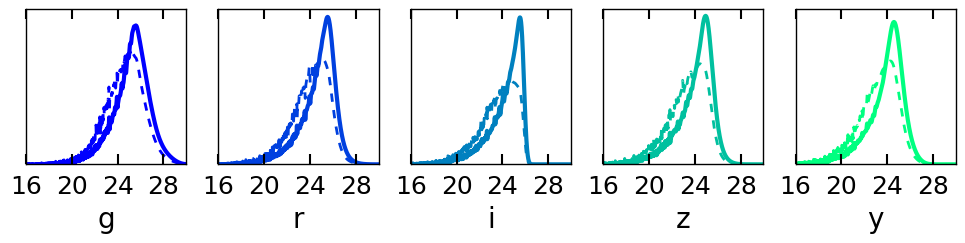
\includegraphics[width=\textwidth]{mag_dist_sel.png}
\end{center}
\caption{Normalized asinh magnitude distribution of selected galaxies. Training set (dashed), testing set (solid).
}\label{fig:mag}
\end{figure*}

\begin{figure}
\begin{center}
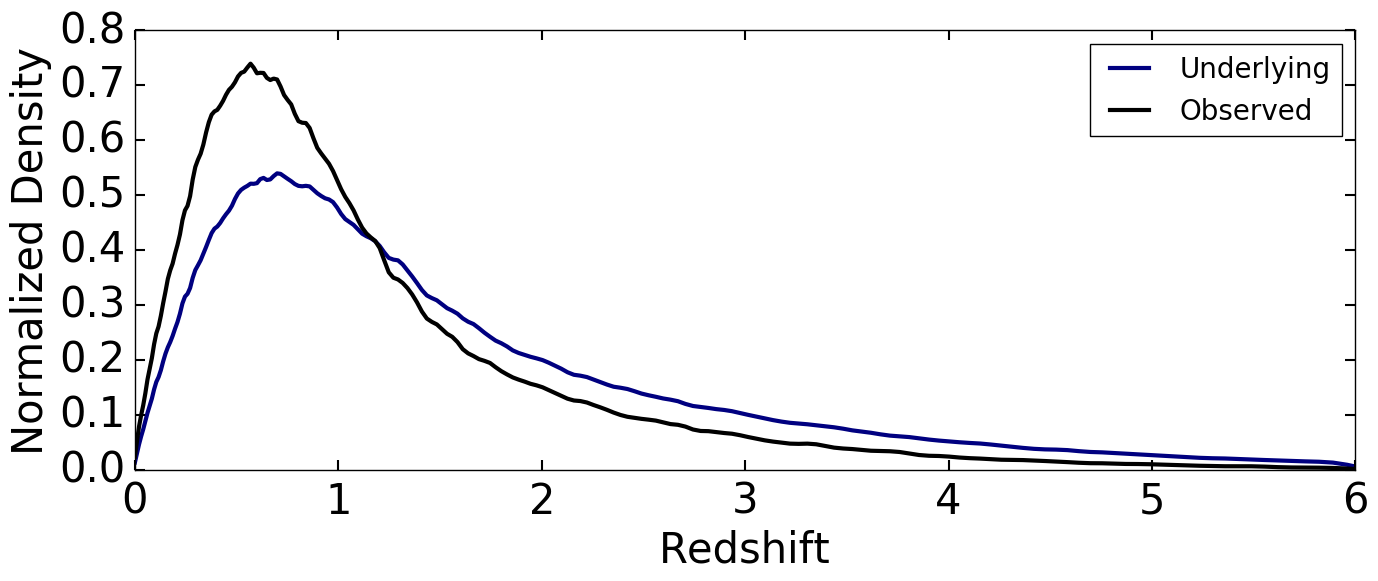
\includegraphics[width=0.48\textwidth]{z_dist.png}
\end{center}
\caption{Redshift distribution of the parent sample (black) and observed sample (blue).
}\label{fig:redshift}
\end{figure}

\begin{figure}
\begin{center}
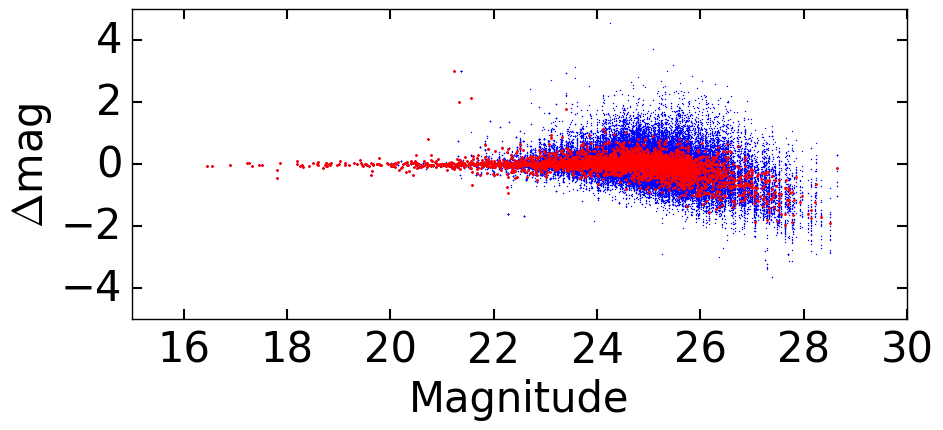
\includegraphics[width=0.48\textwidth]{mag_impute.png}
\end{center}
\caption{Imputed photometry (converted to asinh magnitudes). Random draws are shown in blue, median quantities in red.
}\label{fig:mag_impute}
\end{figure}

\begin{figure}
\begin{center}
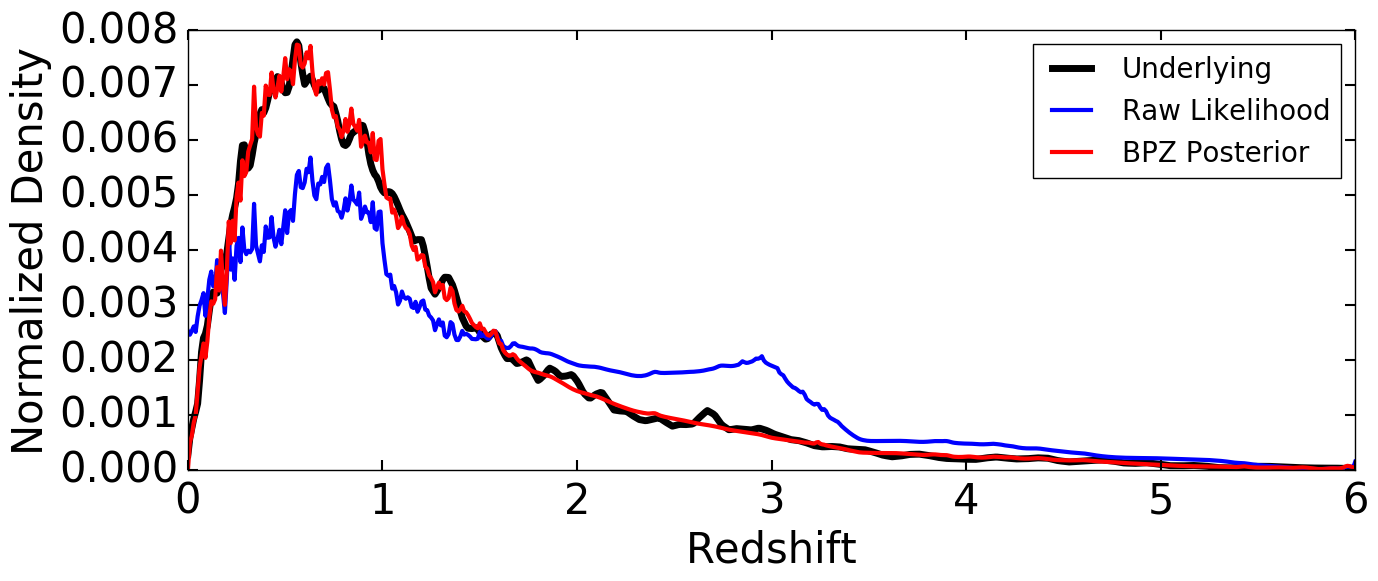
\includegraphics[width=0.48\textwidth]{z_fits_model.png}
\end{center}
\caption{Redshift distribution derived through template-fitting (noiseless model photometry). The raw likelihoods are shown in blue, the BPZ-computed posteriors (no mismatch) is in red.
}\label{fig:bpz_fits}
\end{figure}

\begin{figure}
\begin{center}
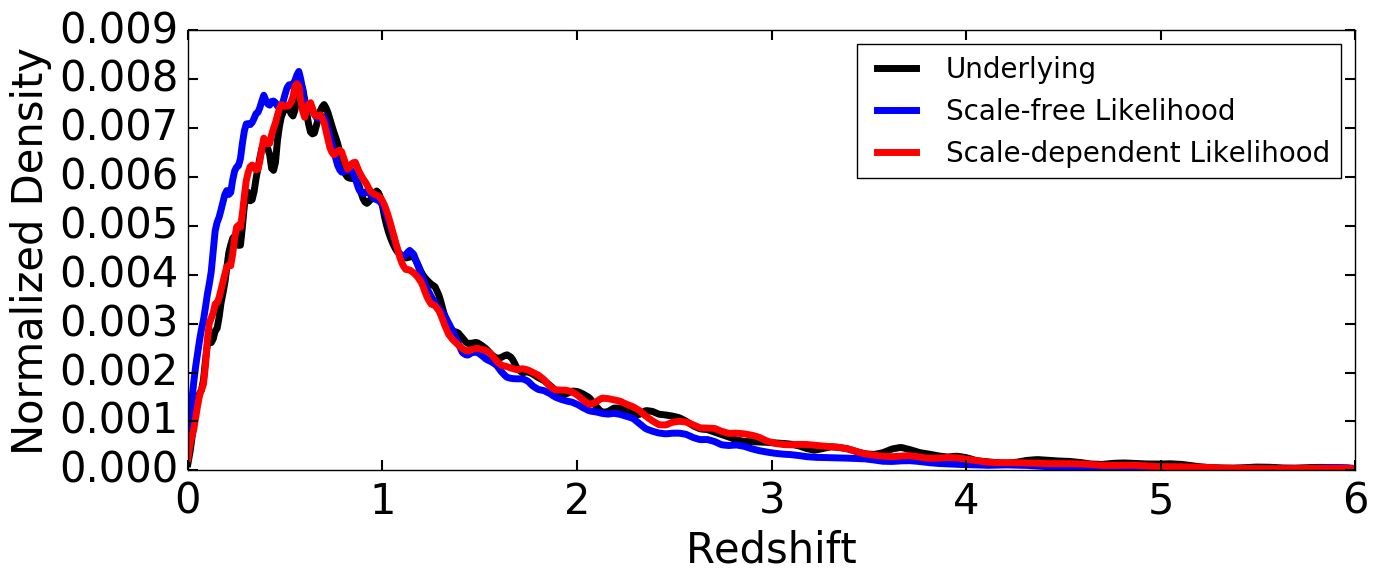
\includegraphics[width=0.48\textwidth]{z_fits_model_sfixed.png}
\end{center}
\caption{Redshift distribution derived from noisy training data assuming a scale-free likelihood (typically used; blue) and a scale-dependent likelihood (red).
}\label{fig:ll_comp}
\end{figure}

\begin{figure}
\begin{center}
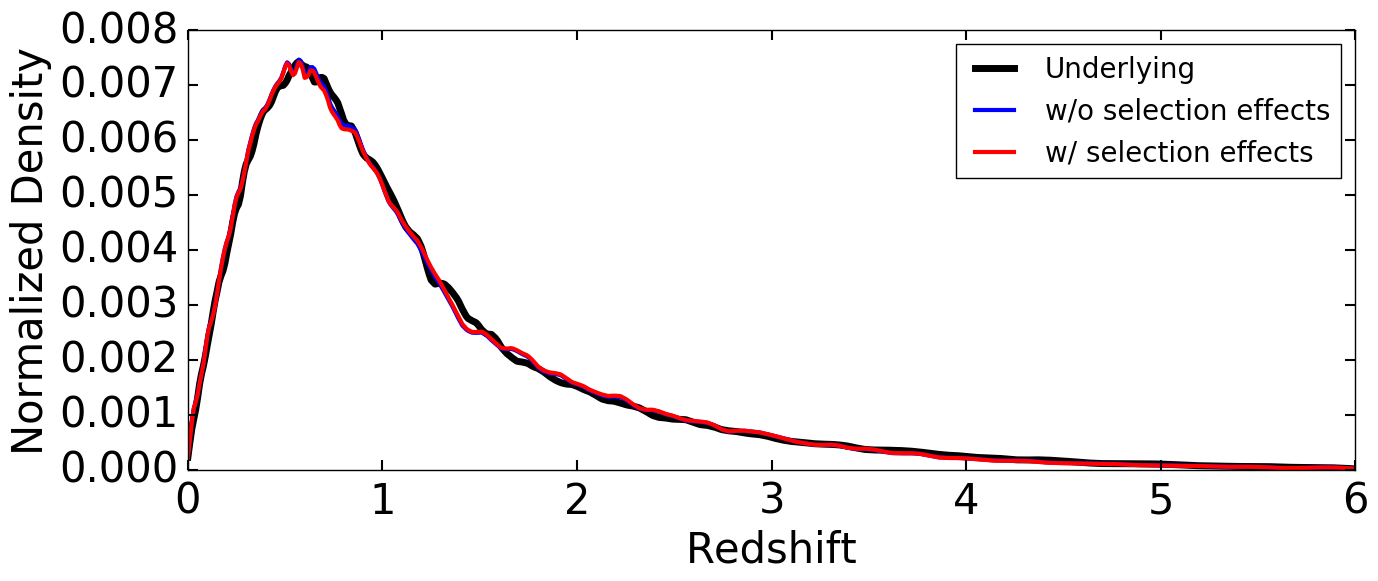
\includegraphics[width=0.48\textwidth]{z_fits_frankenz_sel.png}
\end{center}
\caption{Redshift distributions derived from FRANKEN-Z with (red) and without (blue) corrections for selection effects. Effects are minor because the training/testing sets are selected from the same parent sample with similar noise properties. Can elaborate on later.
}\label{fig:redshift_frankenz}
\end{figure}

\begin{figure}
\begin{center}
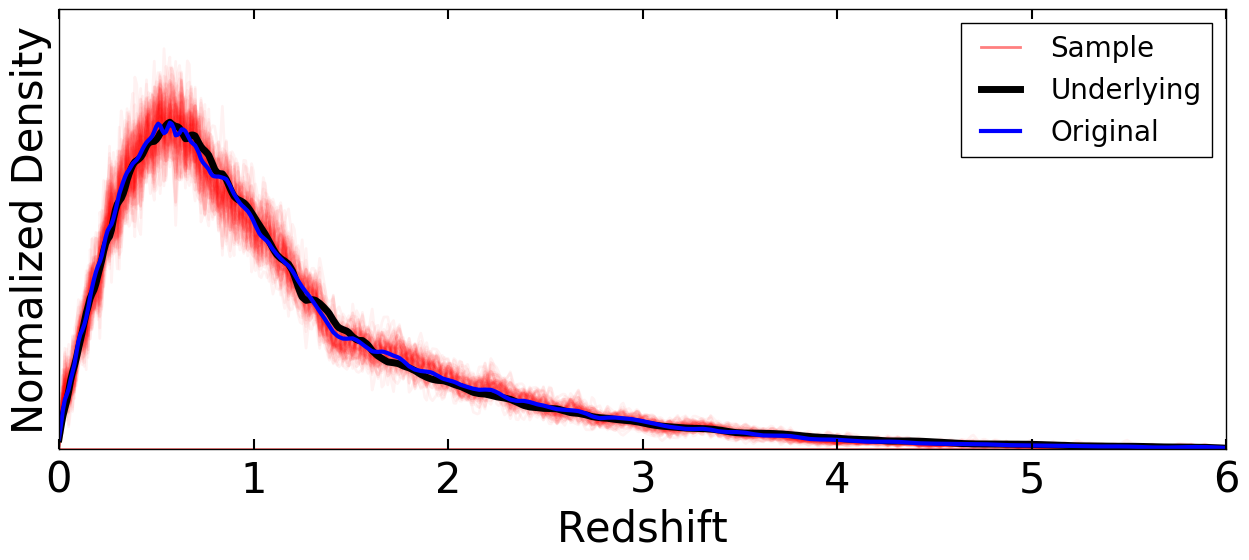
\includegraphics[width=0.48\textwidth]{z_fits_frankenz_sel_hier.png}
\end{center}
\caption{Redshift distributions derived from FRANKEN-Z after including Hierarchical Bayesian modeling over the training set. Samples from the distribution are shown in red (original in blue).
}\label{fig:redshift_hb}
\end{figure}

\section{Discussion}
\label{sec:disc}

Filler text. Filler text. Filler text. Filler text. Filler text. Filler text. Filler text. Filler text. Filler text. Filler text. Filler text. Filler text. Filler text. Filler text. Filler text. Filler text. Filler text. Filler text. Filler text. Filler text. Filler text. Filler text. Filler text. Filler text. Filler text. Filler text. Filler text. Filler text. Filler text. Filler text. Filler text. Filler text. Filler text. Filler text. Filler text. Filler text. Filler text. Filler text. Filler text. Filler text. Filler text. Filler text. Filler text. Filler text. Filler text. Filler text. Filler text. Filler text. Filler text. Filler text. Filler text. Filler text. Filler text.

\section{Conclusion}
\label{sec:conc}

Filler text. Filler text. Filler text. Filler text. Filler text. Filler text. Filler text. Filler text. Filler text. Filler text. Filler text. Filler text. Filler text. Filler text. Filler text. Filler text. Filler text. Filler text. Filler text. Filler text. Filler text. Filler text. Filler text. Filler text. Filler text. Filler text. Filler text. Filler text. Filler text. Filler text. Filler text. Filler text. Filler text. Filler text. Filler text. Filler text. Filler text. Filler text. Filler text. Filler text. Filler text. Filler text. Filler text. Filler text. Filler text. Filler text. Filler text. Filler text. Filler text. Filler text. Filler text. Filler text. Filler text. 

\section*{Acknowledgements}

JSS would like to thank Tansu Daylan, Ben Hoyle, Song Huang, Harshil Kamdar, Jae Hyeon Lee, and Alex I. Malz for insightful discussions. JSS is grateful for financial support from the CREST program, which is funded by the Japan Science and Technology (JST) Agency. This material is based upon work supported by the National Science Foundation Graduate Research Fellowship Program under Grant No. XXX. Any opinions, findings, and conclusions or recommendations expressed in this material are those of the author(s) and do not necessarily reflect the views of the National Science Foundation.

%%%%%%%%%%%%%%%%%%%% REFERENCES %%%%%%%%%%%%%%%%%%

% The best way to enter references is to use BibTeX:

\bibliography{photoz}

%%%%%%%%%%%%%%%%%%%%%%%%%%%%%%%%%%%%%%%%%%%%%%%%%%

% Don't change these lines
\bsp	% typesetting comment
\label{lastpage}
\end{document}

% End of mnras_template.tex